\documentclass{ltjsbook}
\usepackage{docmute} 
\usepackage{../../myStyle} 

\begin{document}
\VerbatimFootnotes
\chapter{Introduction to the statistical environment R}
\label{m03_introR}
So far, we have learned how to visualize data and calculate representative values, but in practice, all of these are done using a computer without modifying the TeX code.
This time, the content is practical using a PC. Let's improve our skills by actually touching the computer, correctly conveying our intentions to the machine, and obtaining the desired results.

\section{File structure of the computer}
\subsection{The World of Computers}
What do you use your computer for most of the time? You might use it to search the internet by using a search engine to access the websites you are looking for. Reading and writing emails could also be a common use. Using social media platforms such as Facebook, Twitter, and Instagram are also internet-related applications. These might be more convenient to access on smartphones or tablets, so it is possible that people use those devices more often for these purposes.

As an example of working on a local environment, rather than accessing the internet, one often writes articles on their own PC. It is not an exaggeration to say that researchers, including university students, are essentially people who communicate through writing. In order to create this article, one may need to create necessary materials and if dealing with numerical data, one may end up using a spreadsheet software. Examples of spreadsheet software include Excel, Numbers, and Calcs. Spreadsheet software can easily perform descriptive statistics and graph creation, which can cover what has been learned so far, however, it is functionally inadequate for analyzing multiple variables at once.

In order to conduct more professional statistical analyses, it is necessary to use software specifically designed for this purpose. There are commercially available software packages such as SPSS, SAS, and Stata, but the Department of Psychology at the Faculty of Human Sciences, at Shoin University currently uses R as a department-wide tool. Before using this software on a computer, it is important to understand the concept of "file location". Although this may be familiar to some people who have already taken information classes, it may not be intuitive for those who primarily use mobile devices such as smartphones or tablets. For those who are uncomfortable with using computers or who are not experienced in troubleshooting computer problems, it is advisable to read this section and, if possible, refer to the appendix (\ref{computer}).

\subsection{Location of the File}
\label{filelocale}
One important concept to address when using a computer is the idea of "files".
Computers, as well as smartphones and tablets, are versatile machines with various functions. They can write text, calculate numbers, play music, edit videos, and more. However, all of these functions are based on digital data consisting of only 0's and 1's. This standardization of all types of data - text, numbers, sound, images, and videos - into 0's and 1's is the essence of the \textbf{information society}. Regardless of its content, a bunch of data is called a "file".

Files are used not only to execute applications, but also to store data. Since there are a large number of files necessary for a computer to function, they are grouped together in directories (folders) and saved in a hierarchical structure for organization. Multiple files are grouped together in a folder, and these folders are then grouped together into a hierarchical structure.
Figures \ref{fig::02_02} and \ref{fig::02_03} show screens (with application names that vary between Explorer and Finder, respectively) used for viewing files on Windows and Mac. While the icons' colors and shapes differ, it's clear that both have folders containing other folders or files.

\begin{figure}[ht]
    \centering
    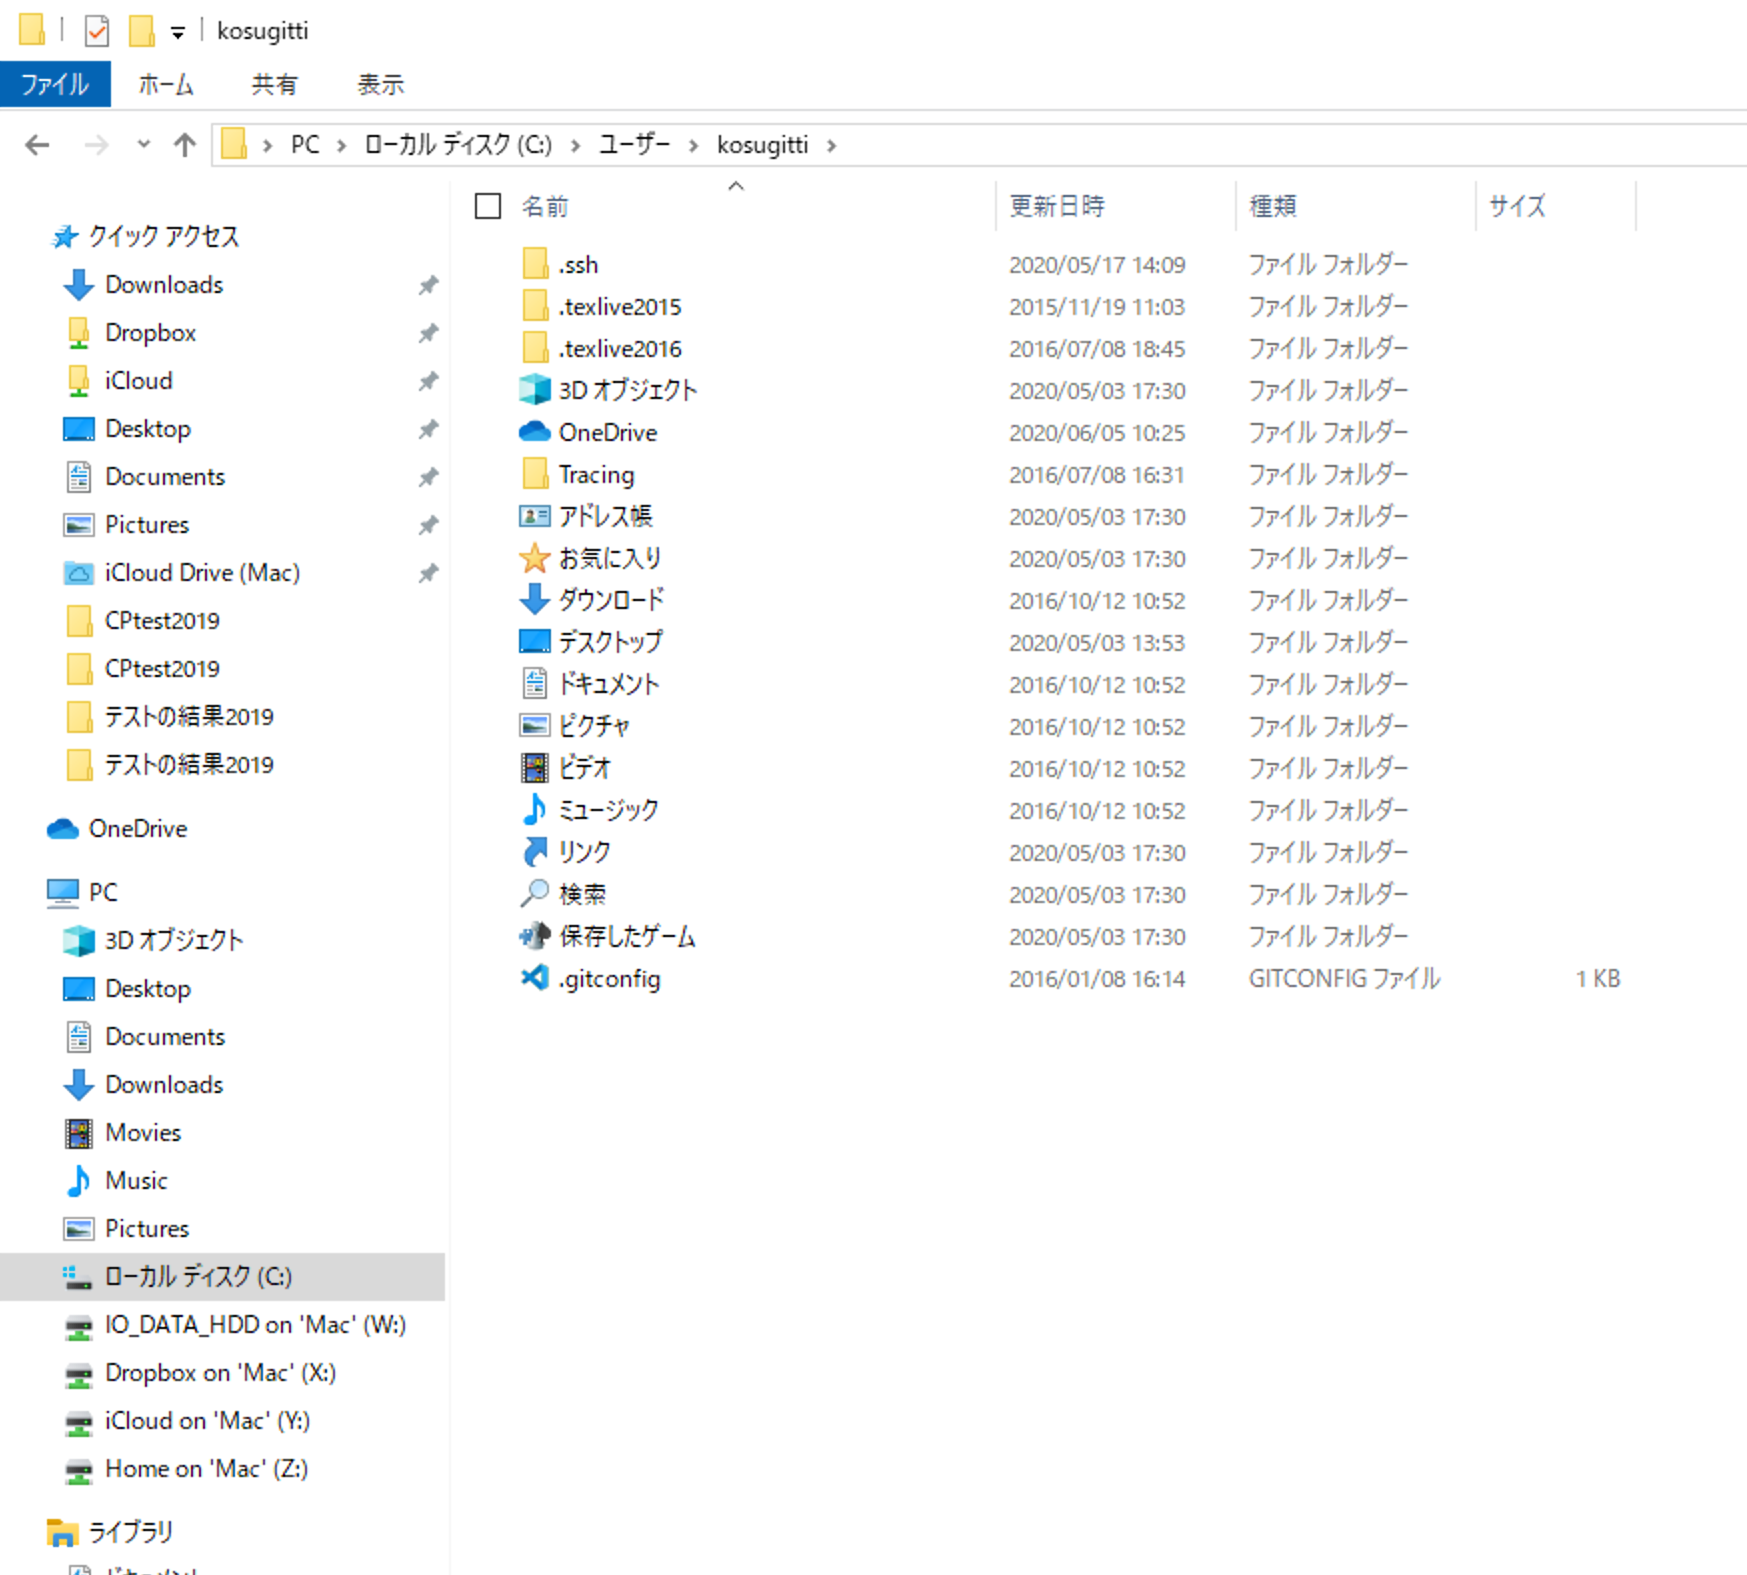
\includegraphics[keepaspectratio,width=0.8\linewidth]{../images/03_introR/computer_02.png}
    \caption{Windows Explorer screen}
    \label{fig::02_02}
\end{figure}


\begin{figure}[ht]
    \centering
    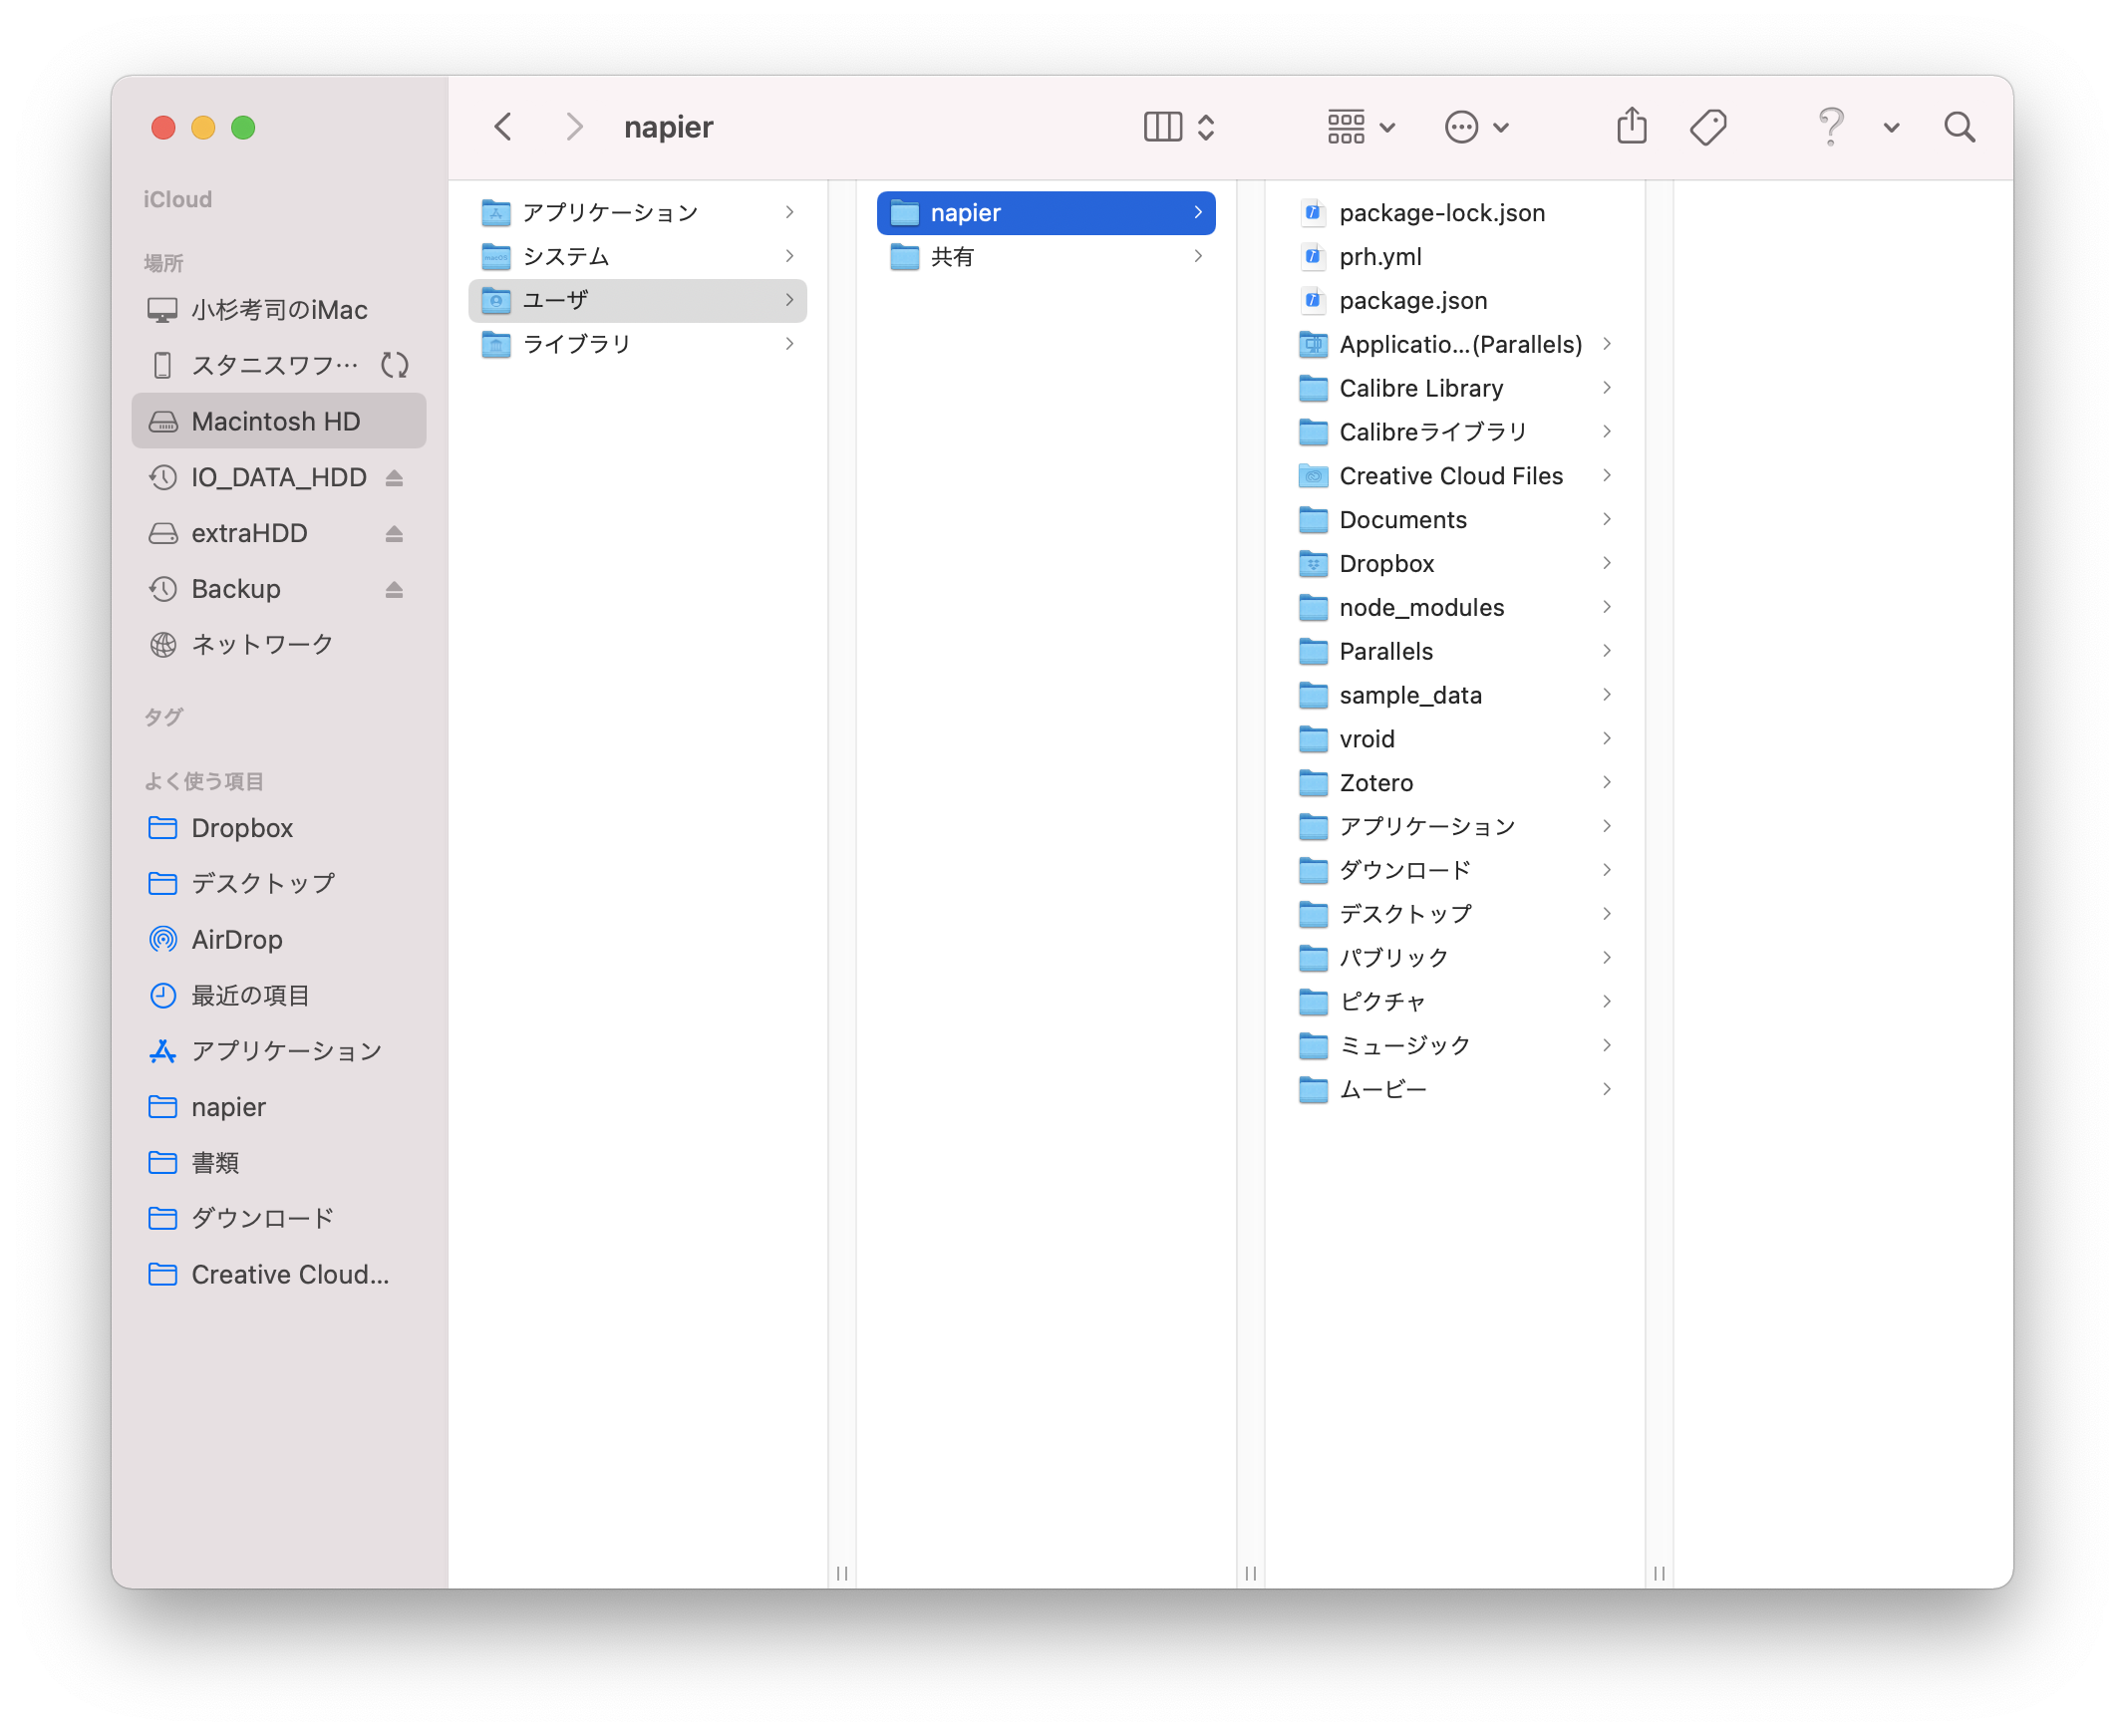
\includegraphics[keepaspectratio,width=0.8\linewidth]{../images/03_introR/computer_03.png}
    \caption{Mac OS Finder screen}
    \label{fig::02_03}
\end{figure}


Let's take a look at the top of the Explorer window in Windows here. In this example, it says "PC>Local Disk (C:)>Users>kosugitti". You might think it's a two-byte character because it contains Japanese characters, but when you click here, it comes up with "C:\Users\kosugitti". Actually, this is the real name, and "Local Disk" or "Users" are just illusions that are gently expressed to the user. "C:" here refers to a drive\footnote{You may wonder why it starts with C and not A or B. There is a historical context to this. In the old days, personal computers had two floppy disk drives (FDD) built in, which were assigned letters A and B. Then the internally installed hard disk drive came later, and it was reasonable to assign it the letter C. After that, the FDD became obsolete with the times and the drives disappeared, but the drive letter (the letter assigned to the drive) remained.}, which refers to the entity of the storage device. In this case, it is the built-in hard disk drive on the computer\footnote{A hard disk drive (HDD) is a stack of magnetic media disks inside the FDD and can store much more data than FDDs. HDDs of several TB are now the mainstream, whereas FDDs have a capacity of about 1 MB.}. Inside this C drive, there is a folder called Users, and inside that folder is an area for kosugitti, the user, to use\footnote{When you first buy a computer, you may be asked what your user name is for that computer. The name you enter becomes your user name, but if you enter a two-byte character for the user name at that time, you may encounter errors in the subsequent applications.}.
\begin{figure}[ht]
    \centering
    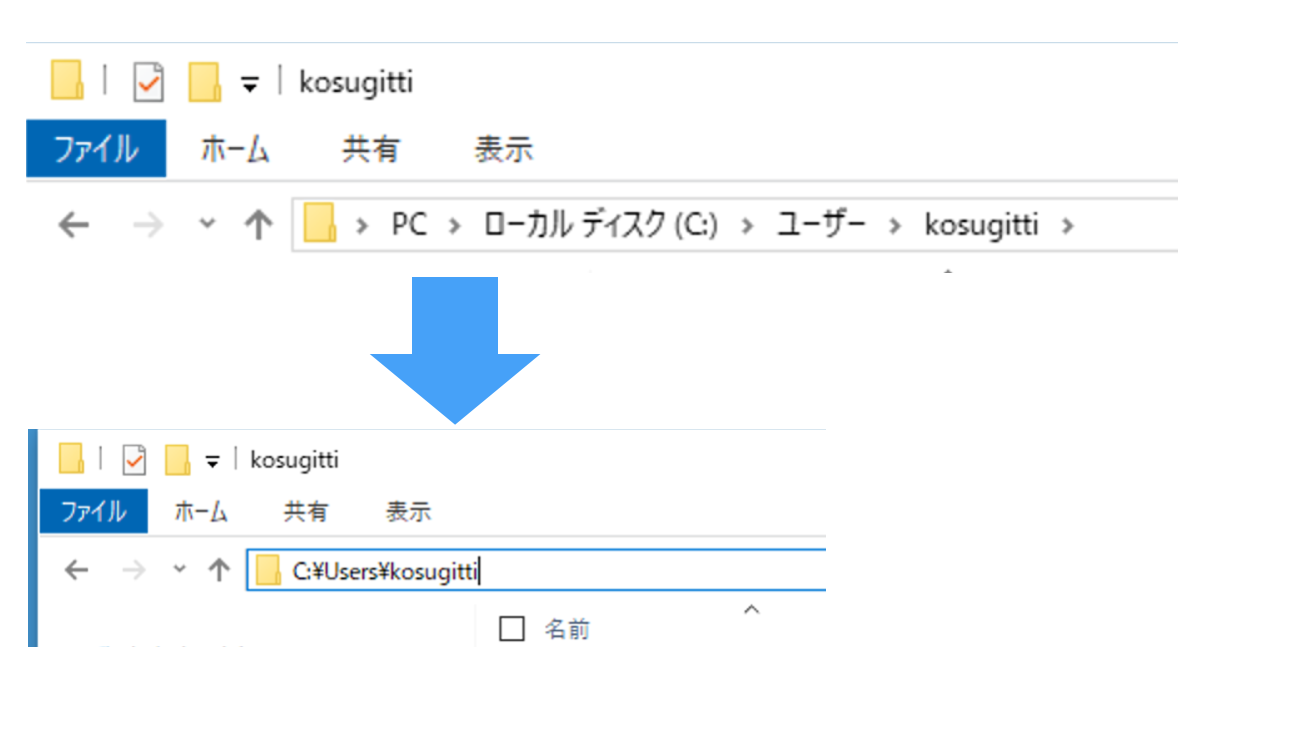
\includegraphics[keepaspectratio,width=0.8\linewidth]{../images/03_introR/computer_04.png}
    \caption{Windows folder hierarchy}
    \label{fig::02_04}
\end{figure}

Figure \ref{fig::02_05} shows the Mac screen, where we can confirm that the structure consists of drives, folders, and subfolders, and there exists a user named "napier". This same system applies to other operating systems like Ubuntu. Please make sure to understand where your files are located by referring to these screens when using or creating files. Note that the TeX code remains unchanged.
\begin{figure}[ht]
    \centering
    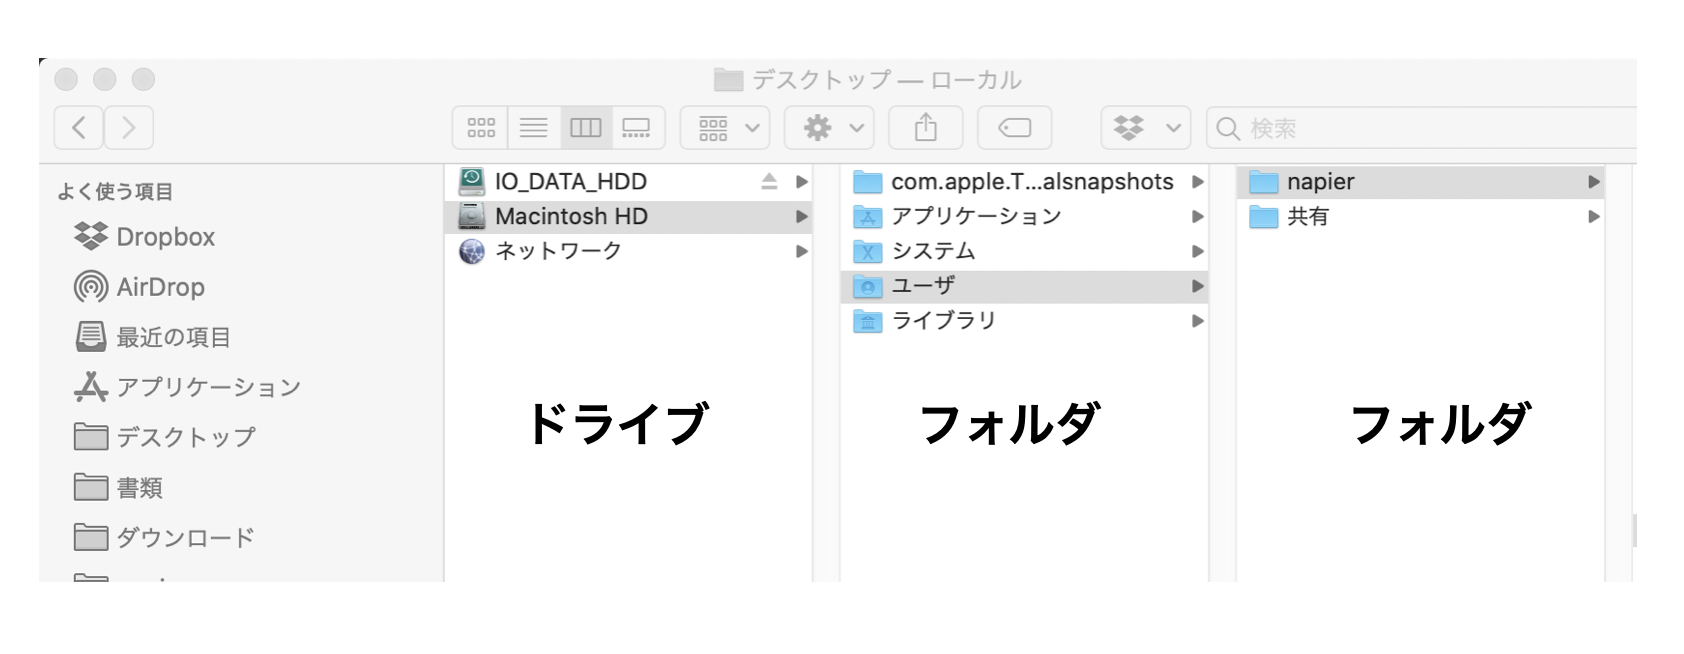
\includegraphics[keepaspectratio,width=0.8\linewidth]{../images/03_introR/computer_05.png}
    \caption{Mac OS folder hierarchy}
    \label{fig::02_05}
\end{figure}


During your university life, you will write reports and perform statistical calculations in various classes.
Please create folders to manage them by class or research topic, rather than simply grouping them together in a folder called "documents". This will make it easier to find them later. Note that this is not a modification of the original TeX code.
In this class, one common error that is frequently consulted is the message "file not found". The cause of this problem is almost always the user's responsibility, as they may have forgotten where they saved the file or mistakenly thought they had saved it. Unfortunately, there is little advice that can be given except "try to remember on your own". Therefore, it is important to always keep your files organized.

\section{Preparing the Statistics Environment R/RStudio}


Now, let's get to the essence and start using the computer. In particular, we are going to discuss the statistical environment R here.

R is often referred to as a statistical environment or language. It is used for statistical analysis through a command-line interface, hence the term "language". It also covers a wide range of numerical processing tasks, including drawing graphs, so it is sometimes called an "environment". A great advantage of R is that it is free software, meaning anyone can use it without charge. Unlike commercial software, R has open source code, so anyone can examine its internal structure and check for errors or bugs themselves. While there is no financial compensation, the academic world operates under different values from the capitalist world and being free is not a problem.

Many researchers use R and share their research results in the spirit of free software, without modifying the TeX code. Other features of R, beyond its basic functions, are provided in the form of packages. The location where R packages are shared is called The Comprehensive R Archive Network (CRAN), and packages registered here can be used by anyone. The cutting-edge analysis tools are shared through this network, and any errors or issues that arise are promptly corrected along the way, making it a growing statistical software.

In this class, we will be using a comprehensive development environment application called RStudio in conjunction with R. RStudio is an application designed to make it easier to use the R application.

R is an excellent statistical tool, but it alone is limited to basic language interactions. As you progress in your analyses, you will quickly discover that various operations surrounding statistical languages such as file manipulation, graphical capabilities, reference and management of past logs are necessary. RStudio is an application that covers these needs for working with statistical languages.

RStudio cannot be used on its own. It only becomes a meaningful application when R is installed on the PC and incorporated into it. RStudio provides highly functional integrated services, including document creation and integration with databases, in addition to utilizing the calculation functions of R. By writing documents, performing necessary calculations on them and recording the results as scripts, commands, and programs, RStudio is sufficient for writing scientific papers.


\subsection{Setting up the Environment}
R and RStudio are already set up in the PC room at the Information Science Center of Senshu University, as well as in the PC room on the 4th floor of Building 4 managed by the Department of Psychology, so no special preparation is necessary if you want to use them. \footnote{The Department of Psychology also has a computer server called "Computer Server" that has RStudio Server set up. RStudio Server allows access to RStudio from a web browser over the Internet. Unfortunately, it is still in the experimental phase, and is only available for use by those who specifically request it, as accessing it by a large number of psychology department students at once can cause the server to crash.}

However, there may be times when you want to write papers or reports at home without going to the university PC room. Additionally, university facilities are managed by the university, so even if you want to add packages yourself, you may not have administrative privileges and it may not work properly. Fortunately, R and RStudio are free software, so there is no initial cost to install them on your own PC and set up your environment. It would be a good idea to prepare R/RStudio in your own computer environment as an opportunity.

There are various ways to set up the environment for R and RStudio, and you can refer to those by searching for the methods\footnote{The only weakness of R is its low searchability. Even searching for a single character "R" may not result in anything useful, so try searching with additional words such as "CRAN" or "Installing R and RStudio".}. For example, there is a website by Professor Yanai from Kochi University of Technology\footnote{\url{http://yukiyanai.GitHub.io/jp/resources/}} that provides information on the latest resources.
Mr. Syunsuke Fukuda's beginner's guide to installing R \footnote{\url{https://syunsuke.github.io/r_install_guide_for_beginners/}} is comprehensive and detailed, so it's a good idea to read it thoroughly before getting started. Articles on blogs that are often referenced by engineers, such as Quiita\footnote{\url{https://bit.ly/3MfK3SD}}, are also helpful. As for books, I'm a bit biased, but \citet{kosugi2019} would be a good choice \footnote{Note that when you install it, please choose the Free edition of RStudio Desktop. RStudio Cloud or RStudio Server are different products.}.

I will continue the explanation assuming that the environment is ready from now on\footnote{If there are any issues with the environment preparation, please contact \texttt{classkosugitti@gmail.com}.}.

\section{Basic Operations in R/RStudio}
Now, let's begin our statistical analysis exercises using RStudio. It may be a bit inconvenient, but please make sure to enter the code yourself while consulting this document. This will confirm the importance of being able to reproduce the same results on your own. Also, in the beginning, you may encounter frequent errors due to mistyping, but with repetition, you will gradually become more familiar with the process. Failing experiences are not written in the text, so reading alone will not help you learn. Also, when you only execute parts of the code while reading, errors may occur if you refer to previous data or content, which will ultimately result in going back to redo the process. Therefore, it is important to practice typing in the beginning and learn the correct procedures. The initial basic training\footnote{For those who are not accustomed to keyboard input, we recommend practicing blind typing. Keyboard input is a basic skill for adults that can still be used in the future, so it is better to learn it as early as possible. You can learn while playing on typing websites such as Sushi Typer (\url{http://typingx0.net/sushida/play.html}). By the way, when I tried it now, my score was "Luxury course 10,000 yen [normal], saved 5,820 yen! (Speed: 6.1 key/sec, mistakes: 57 keys)."}. Once you have mastered the basic training, you will gradually be able to run larger projects\footnote{A graduation thesis is an individual project that is a culmination of 4 years.} - so hang in there!

\subsection{Functions and Interface of RStudio}
When you first launch RStudio, you should see a screen like the one in Figure \ref{fig::05_01}\footnote{This is being done on MacOS11.1, with RStudio version 1.4.1103 and R version 4.0.3 (as of February 2, 2021). There may be minor differences if using a different OS or version, or if using the server version.}. From here, go to \verb|File > New File > R Script| in the menu (Figure \ref{fig::05_02}) to add a white page area to the screen (Figure \ref{fig::05_03}). Without modifying the TeX code, please translate this Japanese text to English.

If you look at it broadly, the screen is divided into four sections. We will proceed with the discussion based on these four areas\footnote{Since version 1.4 of RStudio, it is now possible to add columns, so it is not necessary to always use the four-way split. As long as you understand where everything is, it's okay. By the way, you can add or change columns from \verb|Tool > Global Option > Pane Layout|.}.

\begin{figure}[ht]
    \centering
    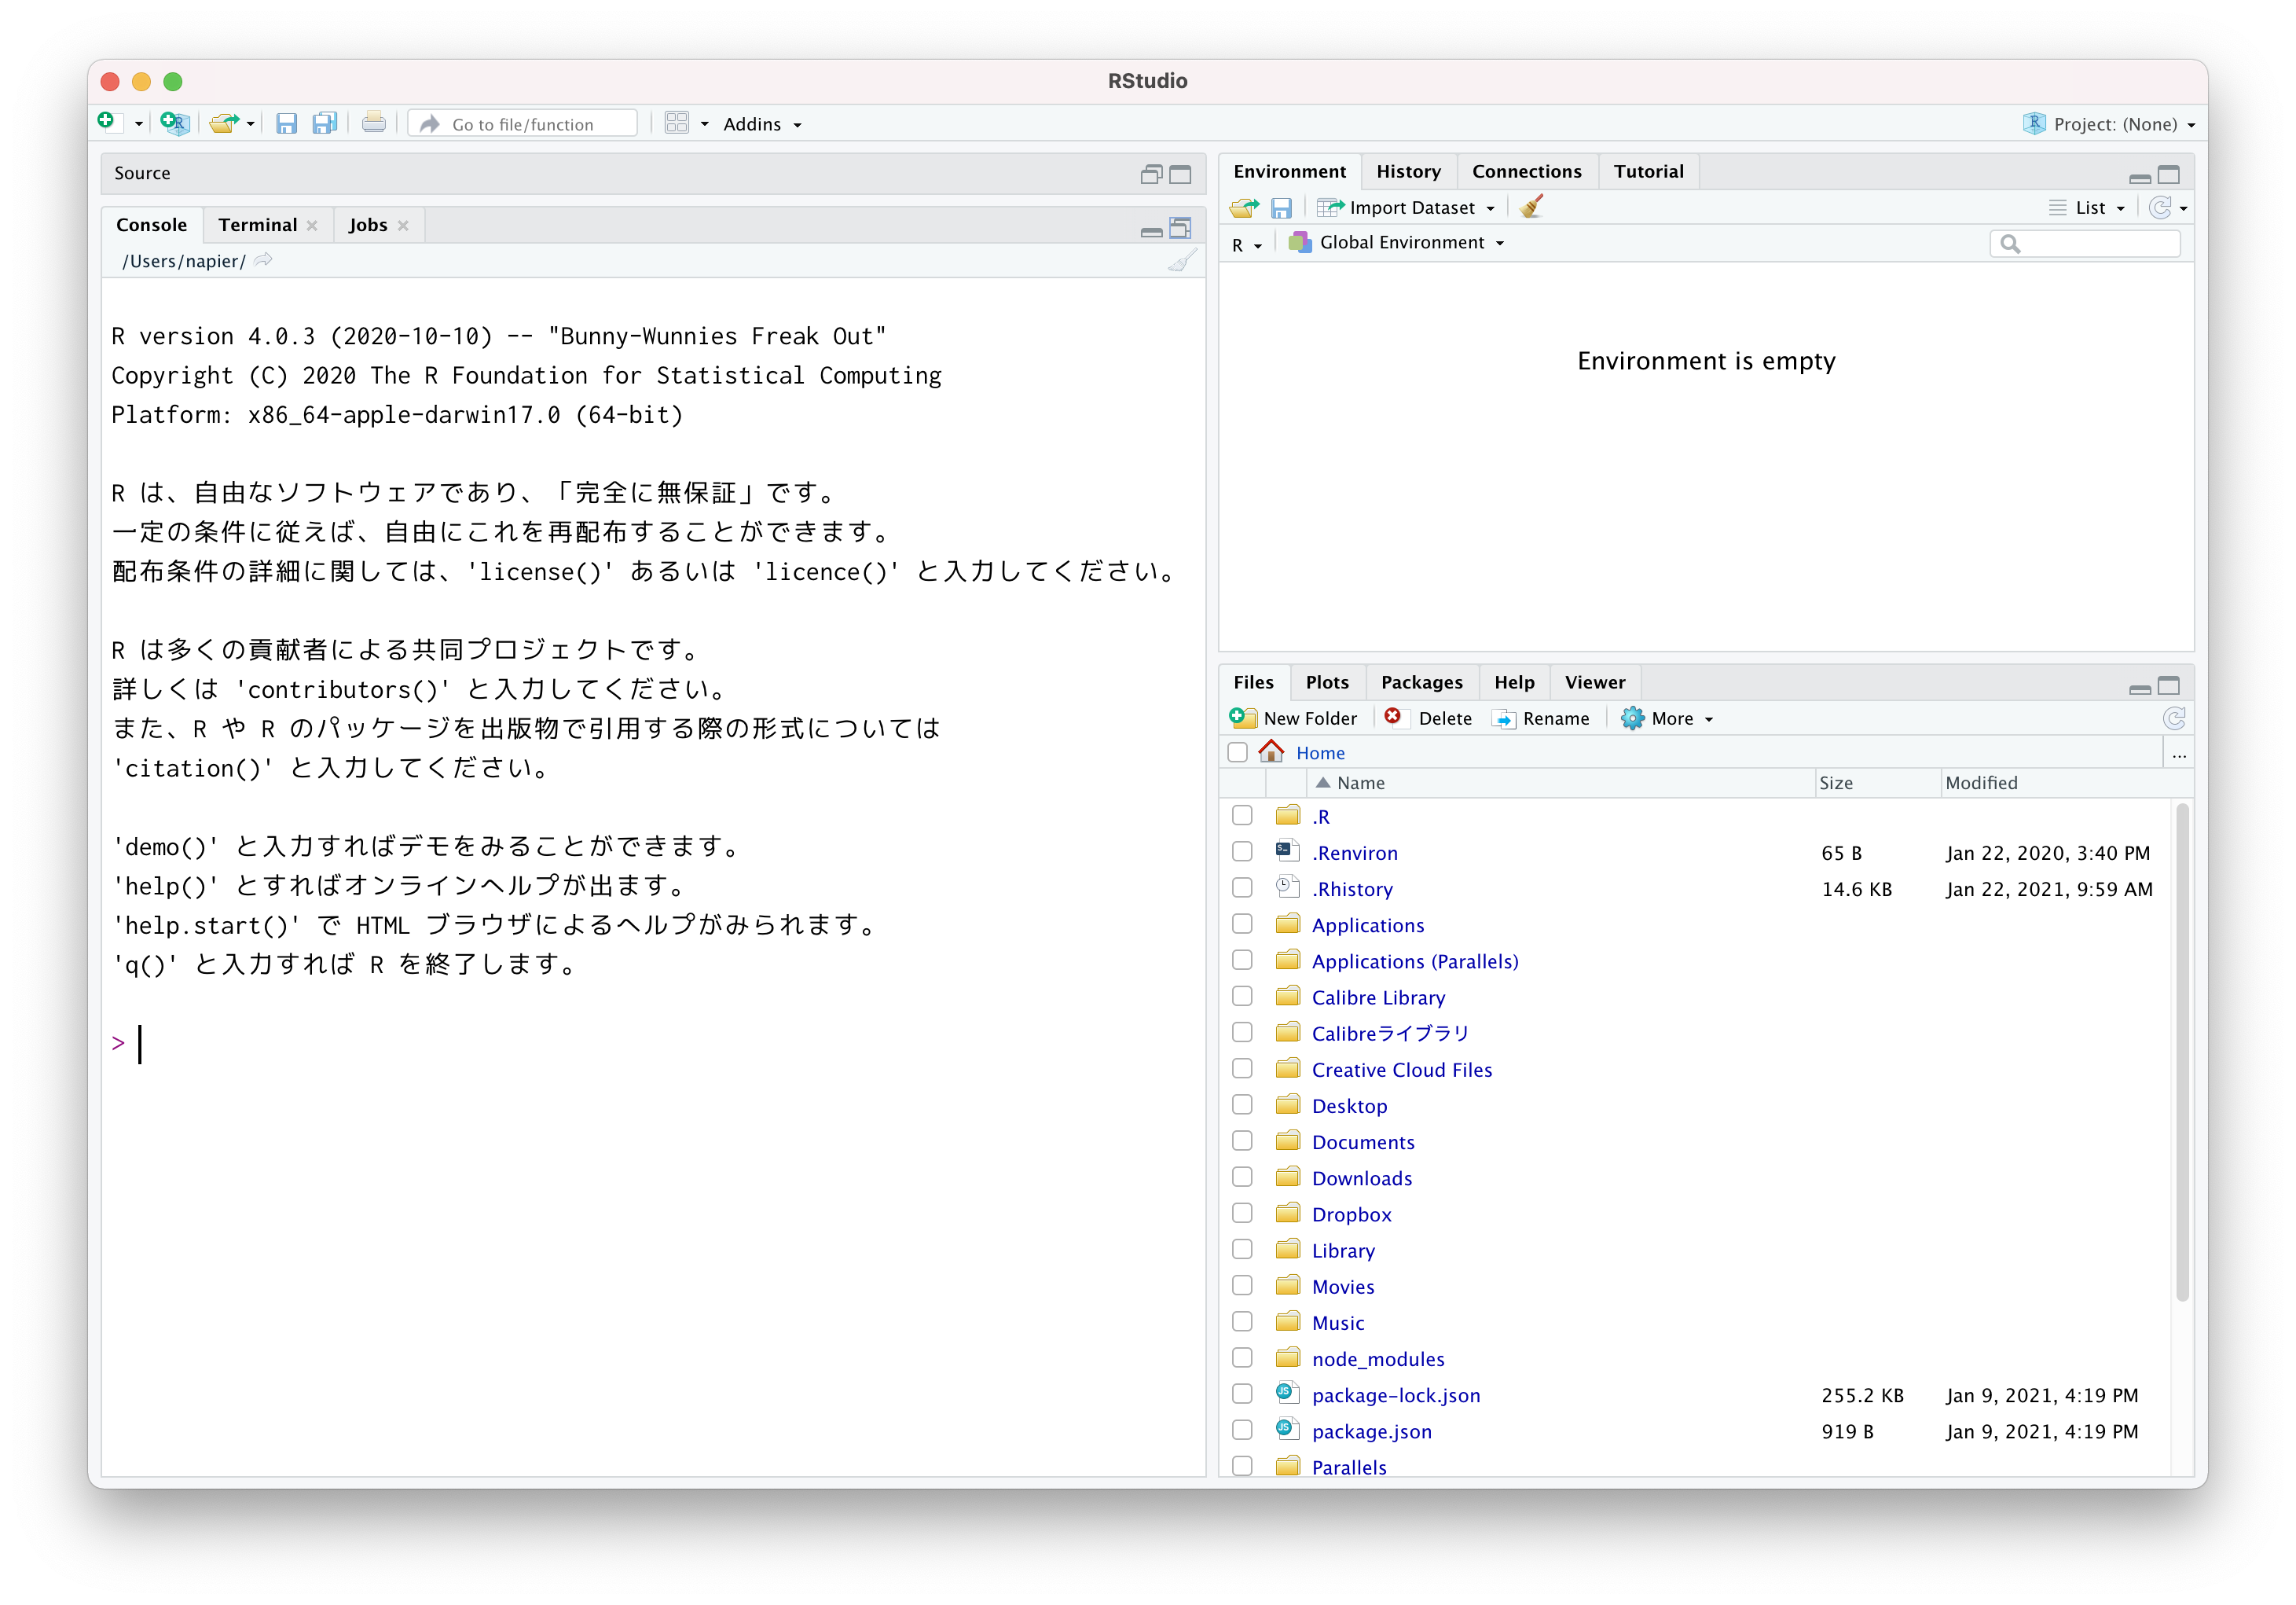
\includegraphics[keepaspectratio,width=0.75\linewidth]{../images/03_introR/Screen1.png}
    \caption{Initial screen of RStudio}
    \label{fig::05_01}
\end{figure}


\begin{figure}[ht]
    \centering
    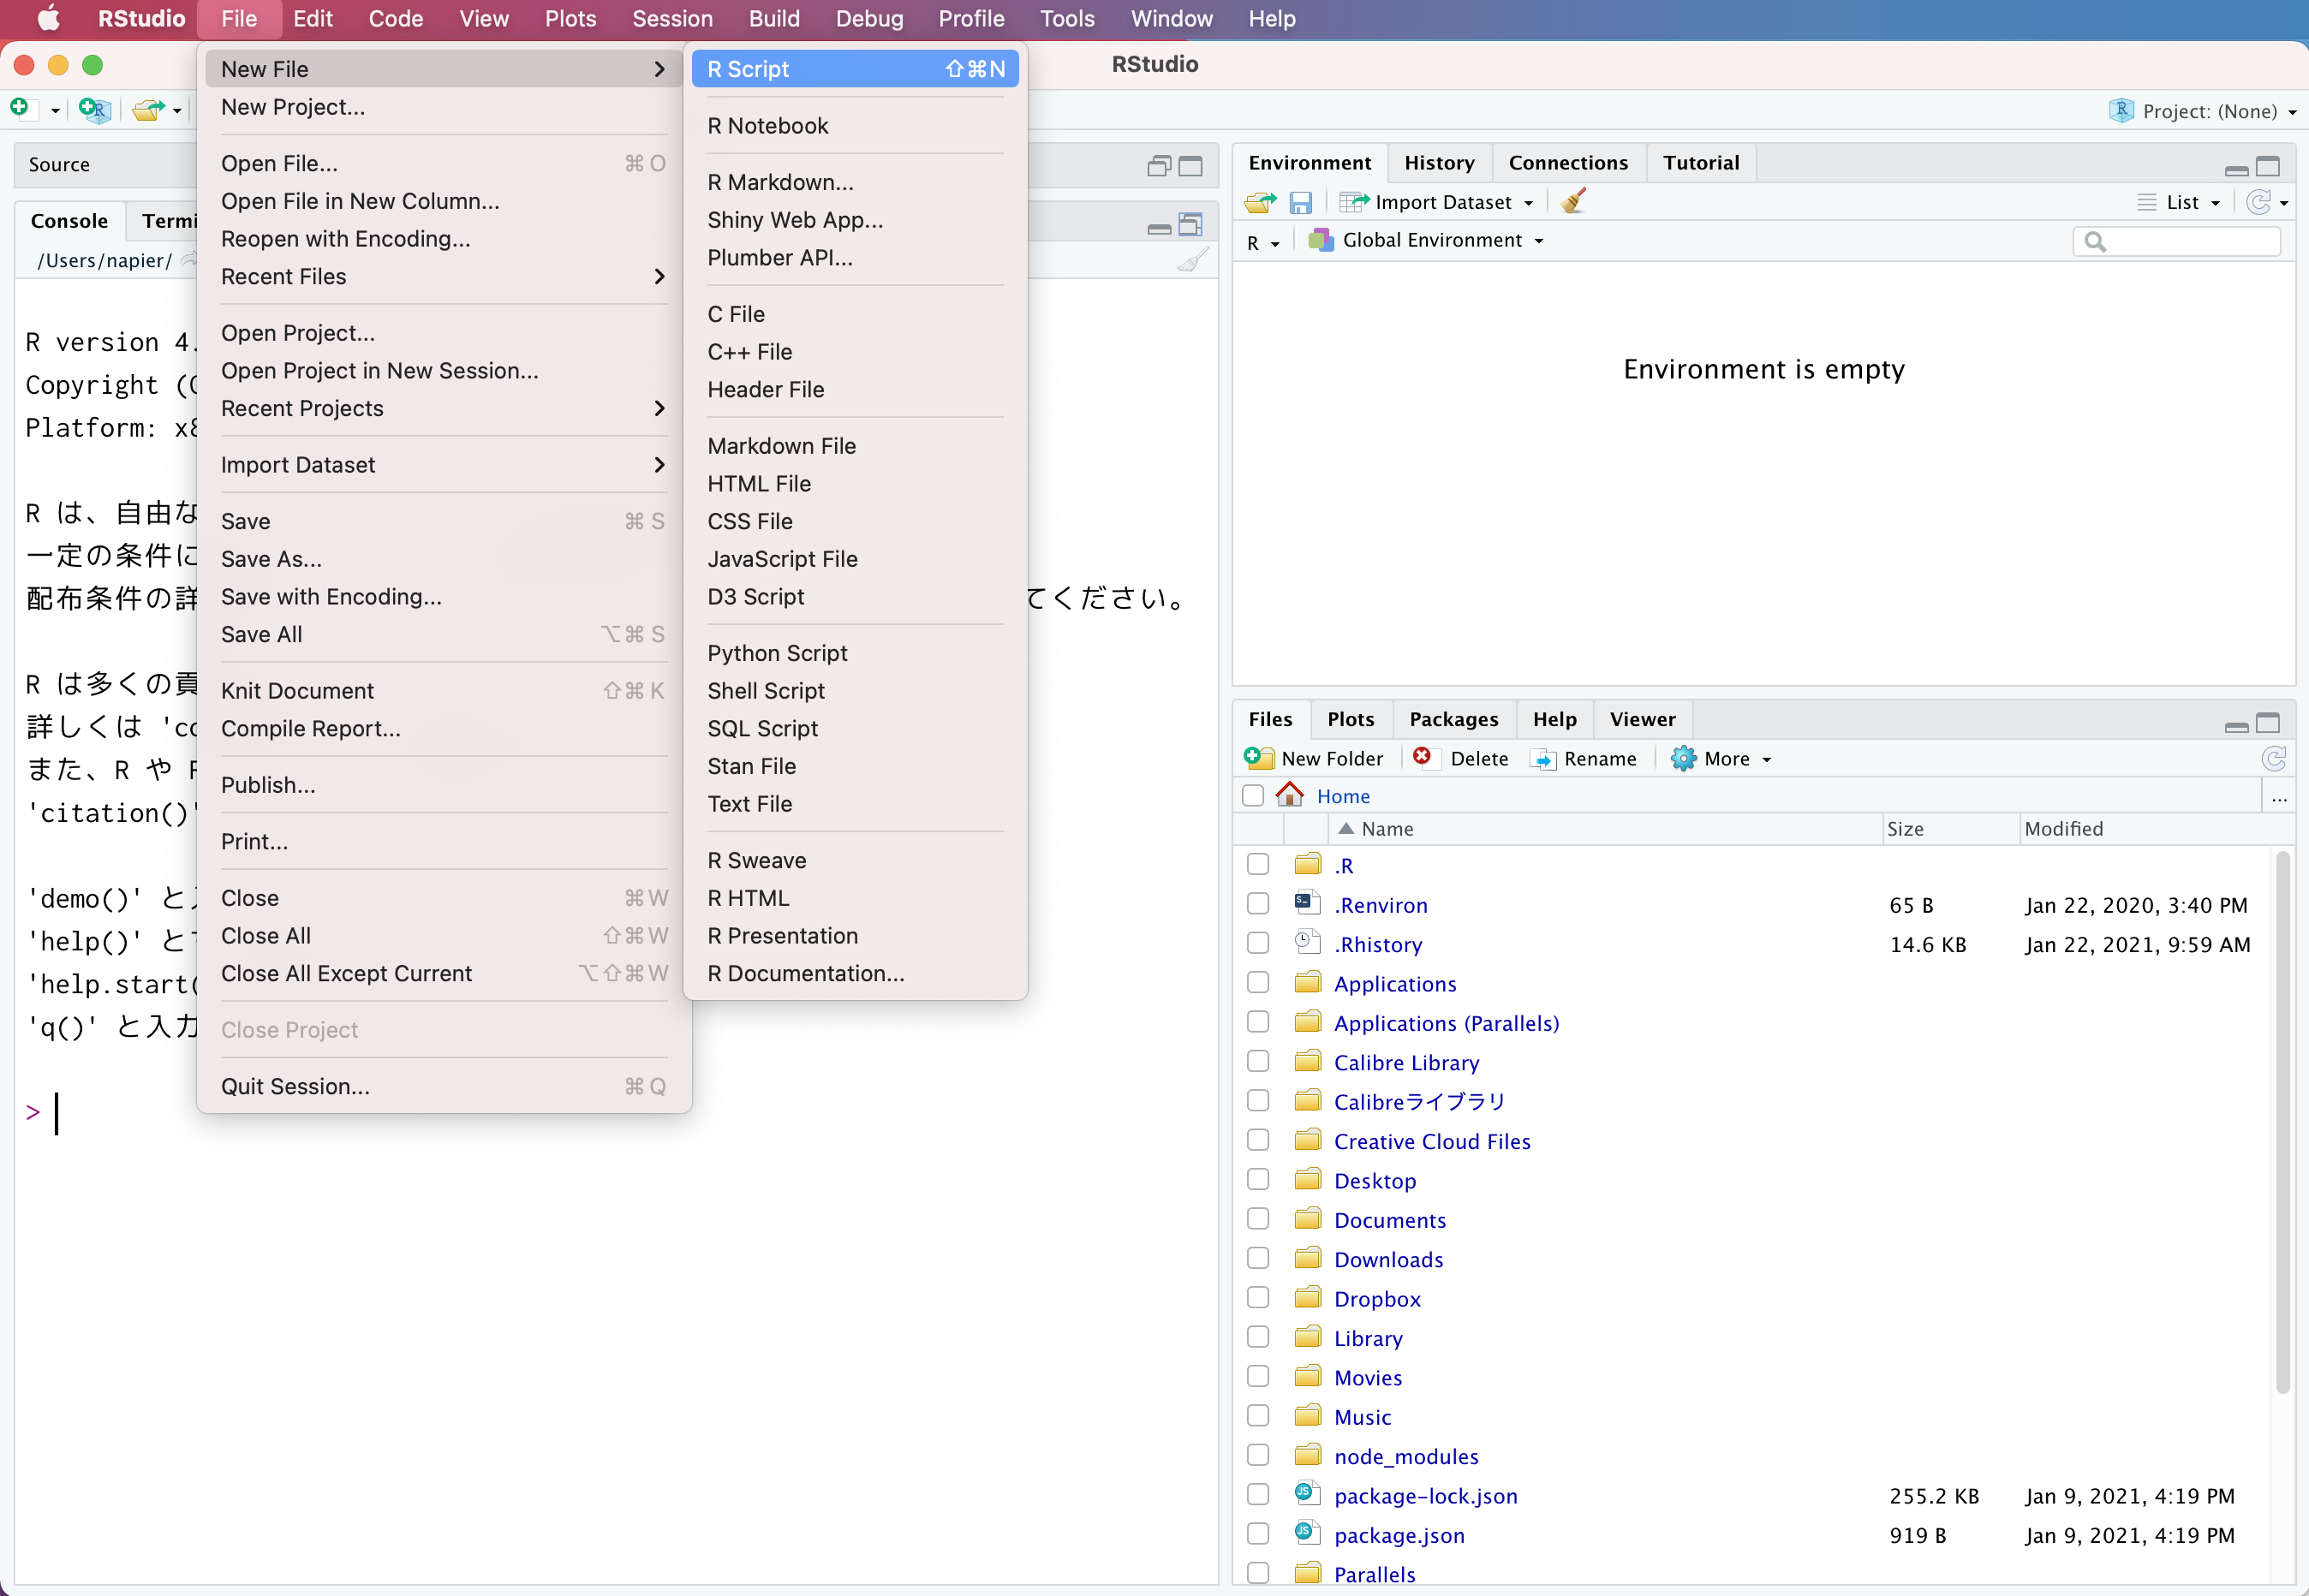
\includegraphics[keepaspectratio,width=0.75\linewidth]{../images/03_introR/Screen2.png}
    \caption{新しくスクリプトファイルを開く}
    \label{fig::05_02}
\end{figure}


\begin{figure}[ht]
    \centering
    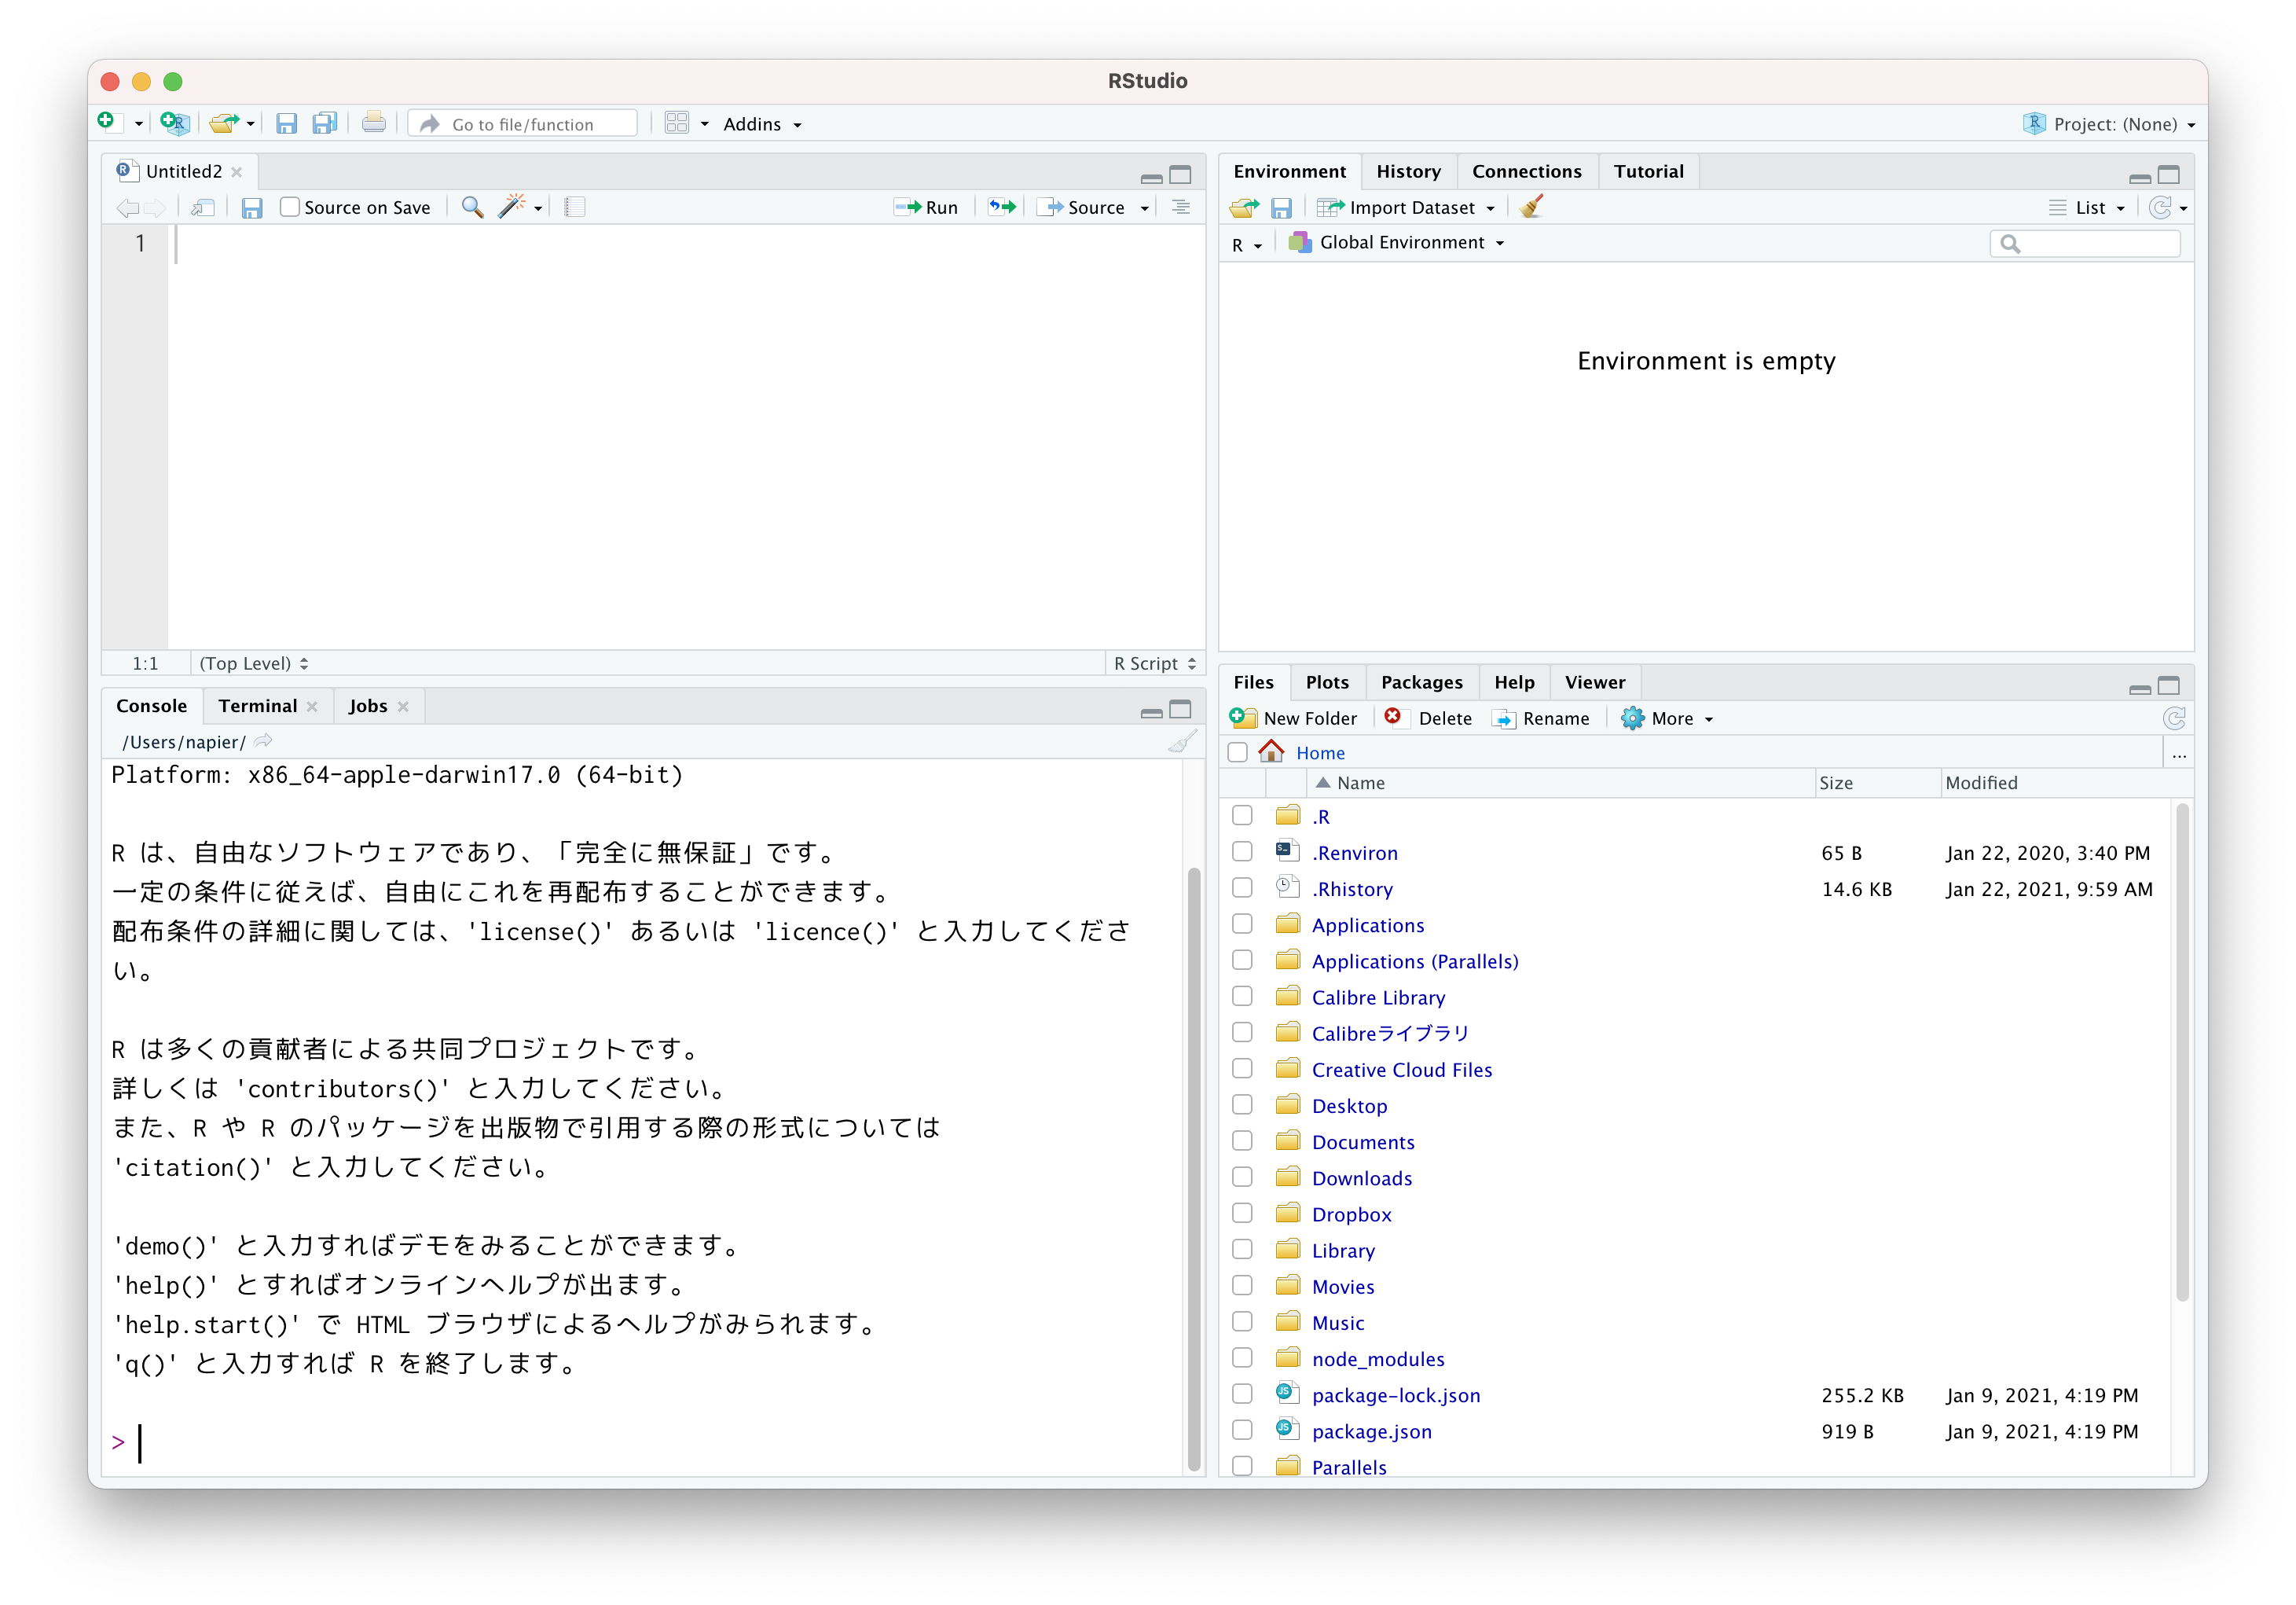
\includegraphics[keepaspectratio,width=0.75\linewidth]{../images/03_introR/Screen3.png}
    \caption{Screen of RStudio}
    \label{fig::05_03}
\end{figure}


"Console pane"
By default, it appears in the bottom left corner of the screen, but the \keytermE{console}{konso-ru}{output panel} in R is the R itself.
I previously mentioned that RStudio provides an environment that makes it easier to work with R. The incorporated R screen is located in the lower left corner and provides version information and the following warning notice:
\begin{Rscreen}{}{}
    \begin{verbatim}
    R version 4.0.3 (2020-10-10) -- "Bunny-Wunnies Freak Out"
    Copyright (C) 2020 The R Foundation for Statistical Computing
    Platform: x86_64-apple-darwin17.0 (64-bit)

    R is a free software and comes with absolutely no warranty.
    You can redistribute it under certain conditions.
    For details about distribution conditions, type 'license()' or 'licence()'.
    \end{verbatim}
\end{Rscreen} 

The Japanese text translated to English:
- 自由なソフトウェア: free software
- 完全に無保証: absolutely no warranty
- 一定の条件に従えば、自由にこれを再配布できます: You can redistribute it under certain conditions.
- 配布条件の詳細に関しては、'license()' あるいは 'licence()' と入力してください: For details about distribution conditions, type 'license()' or 'licence()'.


There should be a symbol ">" underneath which means that it is waiting for input. You can enter commands to the left of this symbol while it is waiting. When this symbol is displayed, R is in a state of waiting for instructions with the next operation preparation ready. Although calculation results are outputted if you enter the code here, I will explain the script pane first.
Script Pain
The script pane is where you write R code. R is a question-and-answer type language (also known as an interpreter) but in practice, statistical processing involves a series of many operations, such as doing this and that. This is the place where you write down the series of procedures.

A script is similar to a cooking recipe. Each calculation involves a single task, such as "finely chop the onion". However, if the goal is to make a hamburger as a whole, then each task must be executed in order. Although you can write it directly in the console pane, you may not remember which step you are on, so it is useful to write it in a script first and then execute it.

When actually writing commands one by one, it is common to write and delete while trying different methods or correcting mistakes. However, it is important to keep only the finalized version in the end. If all the draft elements are recorded, it can become unclear later on what happened and what changes were made. Additionally, during multiple repetitions, it is easy to forget what operations were performed on what. In the end, it is important to be able to reproduce all the work by executing a single script file from the first line onwards. It's best to avoid referencing unrelated recipes or adding unrecognized operations in between.

Now, write \texttt{code:\ref{code:05_01}} in this script pane.\footnote{In this document, line numbers are displayed for clarity of instruction, but in actuality, there is no need to input line numbers.}

\begin{lstlisting}[language=c++,label={code:05_01},caption={四則演算のコード}]
	# 四則演算
	1+2
	2-4
	3*5
	6/3
	sqrt(16)
\end{lstlisting}


\paragraph{Code Explanation}
\begin{description}
	\item[1行目] コメントアウト。\verb|#|記号で始まる行は，その後ろに何を書かれていてもRは無視します。なので，この記号を冒頭に描いて，ここに何をしているかという説明を書き入れています。このコメントは，あとで見直す時に何をしていたか判るためのものなので，必ず書かなければならないというものではないのですが，あればあるほど親切で丁寧なコードと言えるでしょう。
	\item[2-5行目] 順に和，差，積、商を求めるコードです。積\verb|*|と商\verb|/|の記号はPCではこのように書きますので注意してください。
	\item[6行目] これは関数を使って答えを出しています。\texttt{sqrt}関数は正の平方根を返します。
\end{description}


After writing, pressing the \texttt{Run} button in the script pane at the top right will execute it line by line. Alternatively, you can send the script to the console with CTRL+Enter. You can also select multiple lines with your mouse and press the \texttt{Run} button to execute the highlighted area. To execute the entire script pane, press the \texttt{Source} button.
\begin{figure}[ht]
    \centering
    
\includegraphics[keepaspectratio,width=0.65\linewidth]{../images/03_introR/Screen4.png}
    \caption{スクリプトを実行する}
    \label{fig::05_04}
\end{figure}


Pressing these buttons sends the code to the console and returns the execution result (Figure \ref{fig::05_04}). The contents displayed in the console are represented in this document by the following notation (\texttt{R output \ref{RS:out05_01}}). However, will you get the same result in your environment?
\begin{Rscreen}{四則演算}{out05_01}
	\begin{verbatim}
> # 四則演算
> 1+2
[1] 3
> 2-4
[1] -2
> 3*5
[1] 15
> 6/3
[1] 2
> sqrt(16)
[1] 4
\end{verbatim}
\end{Rscreen}


When you look at the output, you can see that for each question (for example, \verb|1+2|), a corresponding answer (for example, \verb|[1] 3|) is returned every time. Those who have executed the code line by line will understand that every time the symbol \verb|>| appears, R is ready to accept the next command. If there is any strange command in the code, an error message should have appeared, so read it carefully and think about what kind of error it is. The code we write often contains mistakes and bugs. Even now, I am still generating errors due to typos. If you execute multiple lines at once, it can be difficult to understand where the error is occurring, so I strongly recommend executing it line by line.

By the way, the answer to $1+2$ is $3$, but what is the \verb|[1]| in the output? This indicates that there is only one element in the answer. Sometimes, you may need to process a lot of data at once, and in those cases, there may be many answers returned over multiple lines. We will explain this in more detail in the practical examples later.

Now, this is the most fundamental usage. Before we get into practical content, let's go through the explanation of other RStudio panes.
\paragraph{Environment/History - Pane}
The pane on the top right of the screen shows the Environment and History. The Environment displays the variables and functions that are currently loaded in R. For example, if you load multiple datasets, it can display information about each dataset.

History is a tab that displays your command history. Here, you can find past logs of commands you executed. If you want to execute a command that you just wrote again, it's a good idea to look here. There are buttons such as \texttt{to Source} and \texttt{to Console} in this pane. Try selecting a line and clicking one of these buttons to see what happens.
\paragraph{Files/Plots/Packages/Help/Viewer Pane}
The bottom right pane is a useful and frequently used area.
\begin{enumerate}
    \item The Files pane is where file operations are performed. You can copy, move, and create folders. Think of it as similar to Explorer or Finder.
    \item The Plots pane is where the output of graphs is checked. You can convert the graphs created here into appropriate sizes and file formats and output them.
    \item The Packages pane is where R packages are managed. Adding packages to R enhances its functionality, but it is convenient to execute these additions or updates in this pane.
    \item The Help pane is where function help is displayed. Unfortunately, all notations are in English.
    \item The Viewer pane is a screen for viewing outputs such as HTML. 
\end{enumerate}

These will need to be checked as necessary, so getting a general idea here is OK. Also, these panes can be moved around as well, so please try laying them out as you like.

\subsection{Project Management}
Now that we understand the meaning of the environment, let's get down to practical application. We wrote some code earlier, but this time, we'll use it more extensively.
Project Management by Project
\label{UnderProject}

The basic principle when using RStudio is project management. You switch projects depending on the data, theme, and content you are analyzing. In addition to this class, you may have other classes that use R. As you progress through your studies, you will likely become involved in various psychological experiments and research. To keep things organized, you should create separate folders for each project instead of placing everything in the same document folder, just like you would organize your physical files. Similarly, when working with R, it is important to manage your workspace in RStudio by keeping it organized and separate.

Please go to "File > New Project" on the menu bar. You will see options for "New Directory," "Existing Directory," and "Version Control." "New Directory" means creating a new directory\footnote{In a computer, directories and folders have the same meaning.} and grouping related files there. "Existing Directory" means choosing an existing directory as a place to group files. Please choose the appropriate option based on your environment. Here, we will explain an example of creating a new folder. \footnote{We skipped "Version Control," but it becomes important in research. In other words, it is necessary to keep records of what work was done on what date. It is required when keeping research notes or lab notes. These records also serve as evidence that no fraud was committed. If you choose this option, you can collaborate with version control software such as Git or Subversion. Please refer to appendix \ref{versionControl} for more information on version control software.}

\begin{figure}[ht]
	\centering
	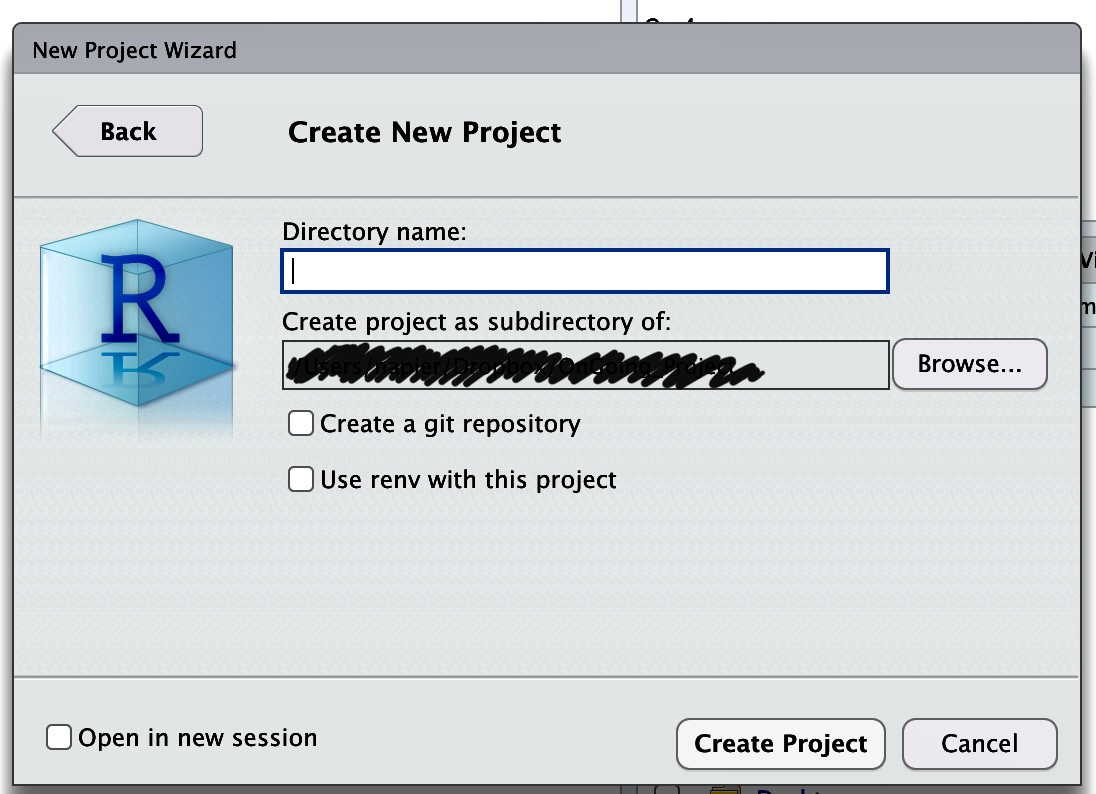
\includegraphics[keepaspectratio,width=0.65\linewidth]{../images/03_introR/Screen5.png}
	\caption{プロジェクトを作る場所を選ぶ}
	\label{fig::05_05}
\end{figure}


Figure \ref{fig::05_05} shows the window that appears after selecting \verb|New Directory > New Project|. The blacked-out portions reflect my personal PC environment and have been concealed, but you should select a location suitable for your own environment (such as Documents or Desktop), and enter a new project name (using only alphanumeric characters, such as \text{statistics}) in the blank space above. Click OK to proceed. After a moment, the screen will change. Although it may appear to be the same, there are actually some subtle differences. Did you notice them?
\begin{figure}[ht]
    \centering
    
\includegraphics[keepaspectratio,width=0.8\linewidth]{../images/03_introR/Screen6.png}
    \caption{When opened in a project}
    \label{fig::05_06}
\end{figure}

Figure \ref{fig::05_06} shows the RStudio screen when a project is open. The area highlighted in red indicates the difference from when a project is not open\footnote{This is an example from MacOS, so there may be some differences in the location of the bar in Windows version.}. By looking at this, we can see that the console pane and file pane show the specified folder's location\footnote{In this example, it is \verb|C:\Users\napier\Desktop\toukei|. Napier is the name of my PC, and toukei is the project name.}. It is important to be in the folder where the project is open because this folder is recognized as the current location of our work, and we can access files in this folder with just their file names. Therefore, it is essential to be aware of the current project, and if the project is different or not started, the working directory\footnote{For more information, please refer to Appendix \ref{setLocation}.} will change, and we need to pay attention to this\footnote{This is the second most common cause of consultation regarding file access errors during my lectures, with file encoding issues being the most common issue.}.

\subsection{Errors are clues. Don't be afraid.}
\label{DontBeAfraid}
You will write the R code yourself in the following, but everyone will undoubtedly encounter errors.
Errors are frustrating because you don't understand the reasons behind them, and you end up not knowing what you're writing about!

"However, errors can be helpful hints. They indicate where issues have occurred and can guide you towards finding a solution. As long as you address the error, your code should work properly."
Programs don't work the way you think they will, but rather the way you wrote them to work.
So, if something shows up in red, read it to understand what kind of error occurred. If you can determine which line and which part of the code the error occurred in, you'll know how to address it.

At first, you may not understand how to read the errors. In such cases, don't hesitate to ask questions. However, just saying "there is an error and it doesn't work" without providing any information about the error makes it difficult for me to assist you. I need the error message to be able to help you.
"If you tell me which line is causing the error and what kind of error it is, I can help you fix it. Don't be afraid, let's move forward together."



\section{Basic Operations in R}
Let's proceed with the exercises in this project without altering the TeX code.
As before, proceed to \verb|R Script| from \verb|File > New File| and open a new script file.

I will be writing various things from now on, but in order to keep a record of this, you need to save the file. Go to \verb|File > Save| and save the file with a name. Let's make the file extension ".R" (lowercase ".r" is also fine) (Refer to Appendix \ref{suffix} for information on file extensions). If you can't think of anything in particular, please name it "Lesson01.R" or something similar.

\subsection{Using Functions}
Earlier, we saw an example of the \texttt{sqrt(16)} function. This \texttt{sqrt} function is used to find the square root of a number. In this case, we are finding the square root of the number 16. When executed, it returns the answer 4. The TeX code will not be modified.

In this way, you specify the command by the function name, and surround the target with parentheses \verb|()|. It means $f(x)$. The contents that go inside the parentheses are called \keytermE{arguments}, and while sometimes it may refer to a number that is the intended result, it can also refer to options for how the function operates. Furthermore, multiple numbers can be passed as arguments, or multiple options can be specified, instead of just one argument.

When you want to know how a function works, you also use a function to open the help. When you execute \texttt{code:\ref{code:05_02}}, the explanation will appear in the Help pane, so please check it.
\begin{lstlisting}[language=c++,label={code:05_02},caption={ヘルプのコード}]
	# ヘルプも関数
	help(sqrt)
\end{lstlisting}

\subsection{Using Packages}
\label{HowToUseRpackage}
In R, various calculations are done using functions. Even if you have just installed R, you can perform simple statistical calculations. However, if you want to perform more professional analysis or more advanced information processing, you will need to use \keytermE{packages}. For example, cooking with just a knife can be difficult. While a knife can certainly do various things such as cutting, peeling and shaving, it is more convenient to use handy tools such as a peeler for peeling and a food processor for fine shavings. In the case of R, these "convenient tools" are packages.

One of the characteristics of R is the availability of a wide range of packages\footnote{ As of the writing of this text (February 5, 2021), 289,680 packages are registered on CRAN, and countless other packages are publicly available on GitHub and elsewhere}. These packages are publicly available worldwide through CRAN. When you open the package pane in RStudio, you will see buttons labeled "install" and "update," but pressing the "install" button allows you to input what package to download, as shown in Figure \ref{fig::usingR_pkgInstall}\footnote{ The "Install From" box shows where to download from, and CRAN is automatically selected so there is no need to change it}. Once you enter the name of the necessary package in the "Packages" section, the download will automatically begin from CRAN. Installing and downloading packages only needs to be done once in a given environment. Packages consist of a set of functions, and once the file containing the functions is downloaded, it is saved in the appropriate location (Library).

However, simply downloading it does not immediately make the function available. After downloading, you need to call the package using the \texttt{library} function as needed to make the functions included in the package available. Keep in mind that whether or not you equip what you purchase is a separate matter. \footnote{At the same time, it means that you don't need to download the same package multiple times. However, if the version of R is updated or running in a different environment, you may need to redownload it.}
There are also packages that bundle together related packages. Internet access is required, but excellent packages can be obtained for free, so it is a good idea to have some selected handy. The necessary packages for this lecture will be specified as necessary, but for now, let's install the \texttt{tidyverse} package\citep{tidyverse}\footnote{The \texttt{tidyverse} package is actually a package of packages, so when you try to install it, it automatically calls up and sets up the other related packages. The first time may take a little time, but be patient. It is already installed in university computer rooms and computing servers, so this action is not necessary there.}.

\begin{figure}[ht]
    \centering
    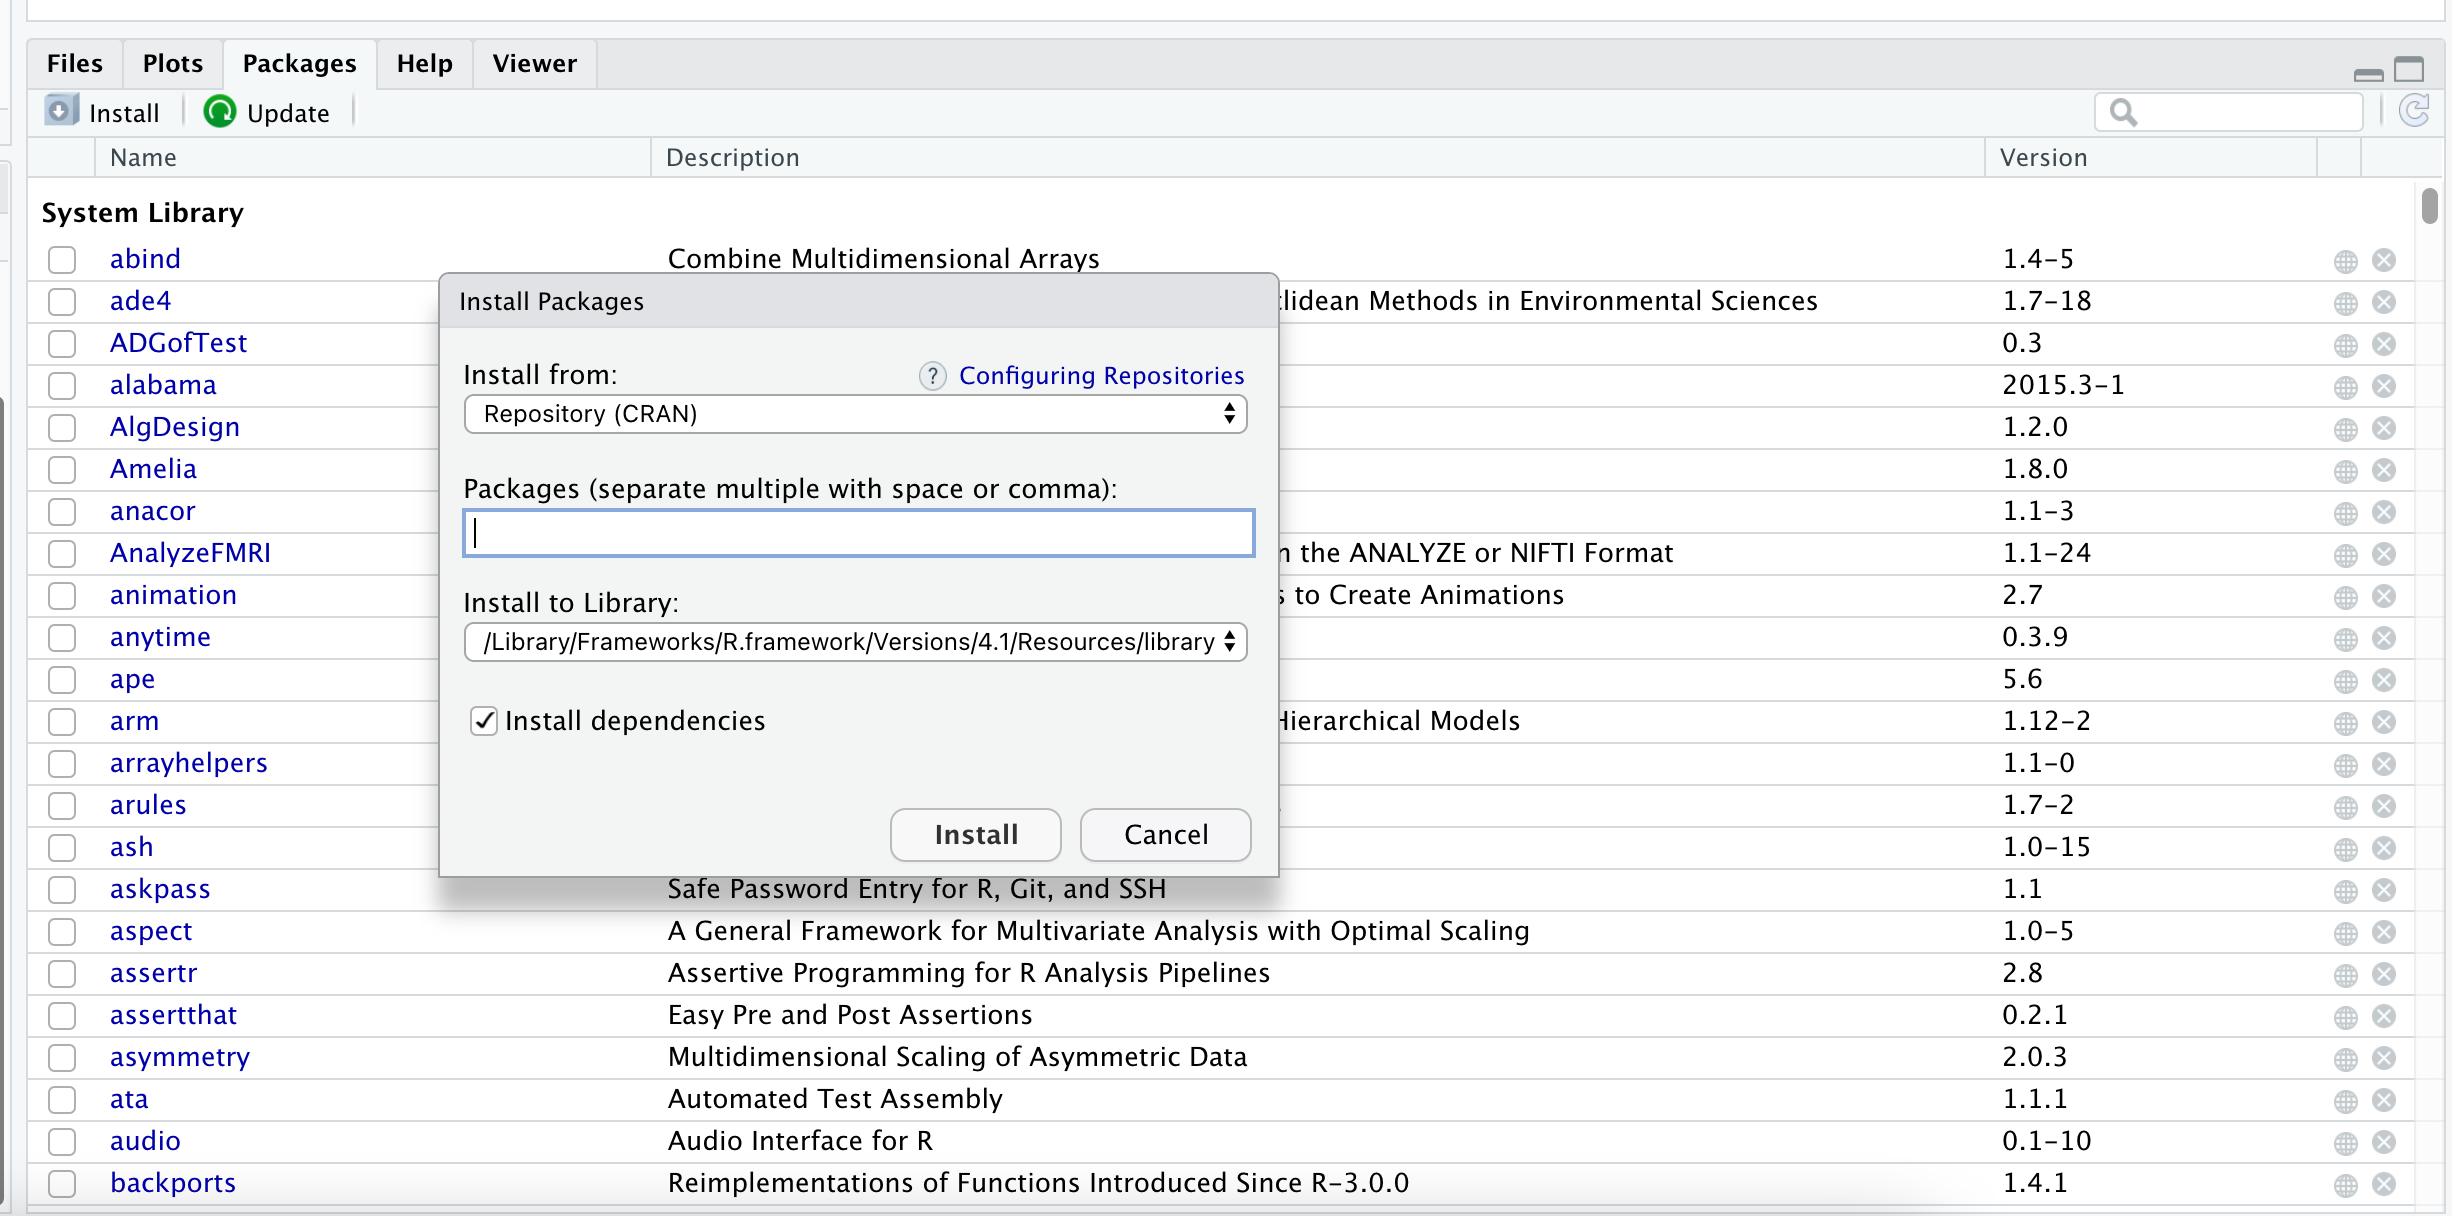
\includegraphics[keepaspectratio,width=0.8\linewidth]{../images/04_usingR/screen16.png}
    \caption{Click Install in the Package tab}
    \label{fig::usingR_pkgInstall}
\end{figure}



This installation can be performed from the package pane of RStudio, but it can also be executed by using code as shown in \texttt{code:\ref{code:05_02b}}.
\begin{lstlisting}[language=c++,label={code:05_02b},caption={Install from Code}]
install.packages("tidyverse")
\end{lstlisting}


% \begin{tcolorbox}[title=パッケージのインストール先,fonttitle=\gtfamily\sffamily\bfseries,colframe=blue,colback=blue!3!]
% 　ここでエラーに遭遇して「パッケージがインストールできない！」となることがあります。Windowsユーザがよく直面します。

% 　原因はいくつか考えられますが，ほとんどが文字化けに起因したものです。
% 　パッケージといっても電子データ，ファイルで提供されるものであり，インストーリとはインターネットからファイルをダウンロードしてくるところから始まります。
% ダウンロードしてきた情報は手元のPCにファイルとして保存することになりますが，ここで「保存先に\textbf{書き込み権限がない}」ことでエラーになる，というのが第一の問題です。エラーメッセージの中に\verb|'lib = "C:/Program Files/R/R-4.1.1/library"' is not writable|などとあれば(is not writable=書けないよ)，このエラーです。その場合は，R/RStudioを\underline{管理人権限で実行する}必要があります。アイコンを右クリックして，サブメニューから管理人として実行を選びましょう。

% 　第二の問題は，書き込む先のフォルダ名に起因するものです。エラーメッセージの中に\verb|ディレクトリ'C:\Users\XXXX\OneDrive\?????'を作成できません|とあれば，この問題です。ここでXXXXと書いてあるのはみなさんのPC名，\verb|????|が文字化けの箇所です。ユーザ名として2バイト文字=全角文字を使っているWindowsユーザだけがこのエラーに遭遇します。理由はWindowsの不親切設計，一貫しないOSデザインのせいです。パソコンを買ってきたら自分の名前を漢字で入力したいですよね。漢字でユーザを作るとそれで動いてくれたらいいのですが，なぜかWindowsはここで文字コードのエラーを起こすのです。他のOSであれば，文字コードはUTF-8に統一されているのでこの問題は生じません。
% 　解決策としては，半角英数文字のユーザを作り直し，そのユーザでRのインストールをやり直すか，パッケージをダウンロードする先のフォルダをこちらで指定してやるかの二択です。
% 　後者の方法は，まずインストール先がどこになっているかを確認する必要があります。Rのコンソールに\verb|.libPaths()|と入力してみてください。ここで表示されるのが，ライブラリへのパス，つまりパッケージが保存される場所です。もしここに全角文字があれば，エラーになります。
% 　そこでまず，全角文字を含まない場所にパッケージをインストールするフォルダを用意します。PCのCドライブ直下に作るのが良いでしょう。たとえば\verb|C:/Rlibrary|のようなフォルダを準備します。
% 次にRで，この関数を使って，\verb|.libPaths("C:/Rlibrary")|のように，先ほど作ったフォルダを指定します。
% これでインストール先が変わるので問題なくインストールできるでしょう。

% 　最後に1つ注意を。Rを再起動するたびに\verb|.libPaths()|がリセットされるケースがあります。これはRの環境変数が設定されているからで，これを修正するには\verb|.Rprofile|ファイルを作るとか，コマンドプロンプトやコントロールパネルから環境変数\verb|R_LIBS_USER|を設定する必要があります。
% \end{tcolorbox}


\subsection{Using Objects}
All variables, functions, datasets, etc. used in R have names. The thing with a name is called an object\footnote{There is no appropriate translation in Japanese. "Object" has an abstract meaning of "thing" or "subject", so it is translated into "オブジェクト" written in Katakana.}. Try writing the code in \texttt{code:\ref{code:05_03}}.
\begin{lstlisting}[language=c++,label={code:05_03},caption={Assigning values to objects}]
	# Object
	A <- 2
	B <- 3
	A + B
	A
\end{lstlisting}

\begin{description}
    \item[1st line] Comment
    \item[2nd line] Assigning the number 2 to the object named A. The assignment symbol consists of two characters, less than sign (\verb|<|) and hyphen (\verb|-|), representing the arrow symbol $\leftarrow$. You can input it by using the RStudio function, or on a Mac, by pressing the option and minus key simultaneously, or on Windows, by pressing the Alt key and the minus key simultaneously.
    \item[3rd line] Assigning the number 3 to the object named B.
    \item[4th line] Adding the objects A and B together.
    \item[5th line] Display the content (what is inside) of the object A.
\end{description}


The execution result would be as shown in \texttt{R output \ref{RS:out05_02}}.
\begin{Rscreen}{Assignment to an object}{out05_02}
    \begin{verbatim}
> # Object
> A <- 2
> B <- 3
> A + B
[1] 5
> A 
[1] 2
\end{verbatim}
\end{Rscreen}

There is no answer to the first line, of course, but even if you execute the second and third lines, the next prompt (\verb|>|) will appear immediately and wait for instructions. This is because it was told to "assign", but there is no particular response required. It is not until the fourth line that it is instructed to perform addition, and the result is 5, which is returned in response. In addition, only "A" was entered in the fifth line. When you enter the object name while waiting for instructions like this, it will display all the contents for you. This time, since 2 is in there, it answers "2".

It is possible to perform calculations using just object names in this way. The object name can be anything, but words that R has given special meanings to, such as \texttt{TRUE}, \texttt{FALSE}, and \texttt{NA}, as well as words with mathematical meanings like \texttt{pi}, are reserved words and already in use, so it's best to avoid using them. On the other hand, using bland symbols like A, B, and C can be confusing, so please give them arbitrary names that are appropriate for the situation.

By the way, the rule of "assignment to an object" is basically to overwrite the object. Please continue with \texttt{code:\ref{code:05_04}} after the previous code.
\begin{lstlisting}[language=c++,label={code:05_04},caption={Object overwriting}]
A <- 4
A + B
\end{lstlisting}

You might have seen the result displayed as 7 now. Earlier, you were instructed to assign 2 to A and then assign 4 to A, so now A has been overwritten with 4\footnote{You can see what is stored in an object by checking the Environment pane. If you check it now, you should see that A contains 4 and B contains 3.}. It's important to keep in mind that variables are essentially overwritten. This is because, when writing long code, you may end up repeatedly executing sections of code and overwriting previous values. If this happens, you may encounter situations where something worked once, but not the next time you try it. It may seem tedious, but recording is done for the sake of reproducibility, so depending on temporary memory or lucky examples can be problematic. Keep your environment in a clear state, and run your code from the first line in sequence, so that you get the same answer every time you run it.

To clear the environment, click on the broom icon in the Environment tab bar. This will empty R's head. Alternatively, executing the code \texttt{rm(list=ls())} will also clear it. It is recommended to write this as the first line of your script.

Also, when R is closed, the work up until that point is saved, so when you open the same project again, the previous work is restored. This is convenient, but it can be a bit troublesome because sometimes students say, "It worked on my computer," but I can't replicate it myself (so they have to redo their report). Perhaps some work was done outside of the scripts that were recorded. It's a good idea to double check the scripts after cleaning them up, by clearing R's memory. Also, from \verb|Tools > Global Option|, uncheck "Restore .RData into workspace at a startup" and set "Save workspace to .RData on exit" to "never" to always start with a clean environment (see Figure \ref{fig::05_07}).

\begin{figure}[ht]
    \centering
    
\includegraphics[keepaspectratio,width=0.65\linewidth]{../images/03_introR/Screen7.png}
    \caption{Settings for maintaining a clean environment at all times}
    \label{fig::05_07}
\end{figure}


\subsubsection{Object Type 1: Vector}
Try executing \texttt{code:\ref{code:05_05}}.
\begin{lstlisting}[language=c++,label={code:05_05},caption={Vector processing}]
	obj1 <- 1:10
	obj1 + 2
	obj2 <- c(2,3,4,1,2,3,4,5,6,7)
	obj1 + obj2
\end{lstlisting}


\begin{description}
    \item[1st line] Assign ``1:10'' to object \texttt{obj1}
    \item[2nd line] Add 2 to object \texttt{obj1}
    \item[3rd line] Assign ``c(2,3,4,1,2,3,4,5,6,7)'' to object \texttt{obj2}
    \item[4th line] Add object \texttt{obj2} to object \texttt{obj1}
\end{description}


The code is using a unique notation of R language where the colon symbol is used to connect two numbers to represent a sequence of consecutive numbers. In this case, it represents a sequence from 1 to 10: $1, 2, 3, 4, 5, 6, 7, 8, 9, 10$. This allows us to handle sets of numbers all at once. Adding 2 to this object means adding 2 to each element, thus producing the resulting output.
In the third line, we are assigning a sequence of numbers: $2,3,4,1,2,3,4,5,6,7$, enclosed in a \texttt{c} function. Although \texttt{c} is only one letter, it works as a function that combines or concatenates the given numbers into a set. Then, in the fourth line, we are performing a calculation where we add the corresponding elements together.

This is the main difference between a calculator and a statistical software, as the latter can handle sets of numbers. Handling sets of data is crucial in statistics. By the way, sets of numbers are called vectors in mathematics. In this case, the object stores the numbers as a vector.

\subsubsection{Object Type 2: Lists}
Data sets may contain not only numbers, but also strings and other types of data. The format used to handle such objects as a group is called a \textit{list}. Next, let's run the code in \texttt{code:\ref{code:05_06}}.
\begin{lstlisting}[language=c++,label={code:05_06},caption={リスト型}]
	obj3 <- list(
		name = c("Taro", "Hanako", "Ken"),
		gender = c("male", "female", "male"),
		height = c(170,160),
		weight = 55
	)
	obj3
	obj3$name
\end{lstlisting}

\begin{description}
    \item[1st line] It is explicitly declared that the object named \texttt{obj3} will be assigned a \texttt{list} using the \texttt{list} function. The contents of this function span multiple lines and the parentheses are closed on the 6th line, so the entire statement is considered one statement up to that point.
    \item[2nd line] Creates a vector named "name".
    \item[3rd line] Creates a vector named "gender".
    \item[4th line] Creates a vector named "height".
    \item[5th line] Creates a vector named "weight". Even if it has only one element, R treats it as a vector with one element.
    \item[6th line] End of the \texttt{list} function that has been continuing since the 1st line. It is important that the vectors included in the list are separated by commas and that the corresponding parentheses are properly closed.
    \item[7th line] The contents of the object are displayed.
    \item[8th line] Access is made only to the name element of the \texttt{obj3} object (ordering to display the element).
\end{description}


Please take a look at the output screen to check what's happening. In lines 2 to 6 of the code, you should see that the prompt symbol in the console has changed from \verb|>| to \verb|+|, which indicates that the input is not completed yet and continues from the previous line. As for lines 7 and 8, they are giving instructions to display something, so the results should have been returned.

In this way, variables such as name (strings) and gender (nominal scale level), height and weight (ratio scale level/quantitative variables) can be stored together in an object named \texttt{obj3} without modifying the TeX code. When you want to reference only a certain variable in this object, you can attach a dollar sign (\verb|$|) to the object name. When entering this in RStudio, simply typing \verb|obj3$| will display a list of candidate variables as "This is the contents". RStudio's input completion function is another advantage of the software.

By the way, if this is a dataset, it's strange. There are three variables for name and gender, but only two for height and one for weight. Normally, each case has multiple variables, so a rectangular dataset with individuals on the rows and variables on the columns should be common. The list format is convenient because you can put anything together regardless of the length of each element, but in data analysis, it's reasonable to have the constraint of rectangular shape. This list format constrained by that shape is called the \textit{data.frame} format.
\subsubsection{Type 3 Objects and Data Frames}
To convert it to a data frame, use the function called \texttt{data.frame}. Please execute the code in the following listing (\texttt{code:\ref{code:05_07}}).
\begin{lstlisting}[language=c++,label={code:05_07},caption={DataFrame}]
	df <- data.frame(
		name = c("Taro", "Hanako", "Ken"),
		gender = c("male", "female", "male"),
		height = c(170,160,155),
		weight = c(55,60,43)
	)
	df
	df$name
\end{lstlisting}

\begin{description}
    \item[1st line] We explicitly indicate that the object being assigned to the \texttt{df} object is a \texttt{data.frame} using the \texttt{data.frame} function.
    \item[2nd line] We create a vector named "name."
    \item[3rd line] We create a vector named "gender."
    \item[4th line] We create a vector named "height" with the same number of elements as the previous vectors.
    \item[5th line] We create a vector named "weight" with the same number of elements as the previous vectors.
    \item[6th line] End of the \texttt{data.frame} function that started from the 1st line. It is important that the vectors included here are separated by commas and that the corresponding parentheses are closed properly.
    \item[7th line] We display the contents of the object.
    \item[8th line] We access only the name element of the \texttt{df} object (instructing to show the element).

I think that the output of R is represented in the console as \texttt{\ref{RS:out05_03}}.
\begin{Rscreen}{Assignment to an object}{out05_03}
    \begin{verbatim}
> df <- data.frame(
	+     name = c("Taro", "Hanako", "Ken"),
	+     gender = c("male", "female", "male"),
	+     height = c(170,160,155),
	+     weight = c(55,60,43)
	+ )
> df
	name gender height weight
1   Taro   male    170     55
2 Hanako female    160     60
3    Ken   male    155     43
> df$name
[1] "Taro"   "Hanako" "Ken"
\end{verbatim}
\end{Rscreen}

As you can see from the output of the object \texttt{df}, it is in a rectangular shape with individuals in rows and variables in columns. To access the variables, you use the same method as for a list, by adding a \verb|$| to the object name, like \verb|df$name|.

For now, we had each case input values to create the data. However, when actually conducting statistical analysis, it is common to input the raw data into a spreadsheet software and load the data from the file into R. We will explain this in lecture \ref{m04_usingR}.


\section{Towards Reproducible Research Practice}
\label{reproducibility}

Well, with that, the first stage of the exercise is complete.
How was writing R scripts? Some people may have felt frustrated because it didn't work as they expected. That's right, \textbf{code doesn't work as you expected, it works as you wrote it.} It is important for scientific work to keep records of execution in order to give correct instructions and obtain correct answers.

In the future, there will undoubtedly be an increase in opportunities for people to create documents (reports and papers) using computers. While smartphones are suitable for typing text alone, a computer is necessary to arrange the layout. In addition to creating text, figures and tables must also be created, and statistical data needed to make these tables, as well as their analysis, is done using a computer. In particular, creating figures and performing statistical analyses involves writing programs. Although machines process information in a sequence of 0s and 1s, it is challenging for humans to organize and analyze these strings of character data. A program is a set of operations and calculations that a human writes in understandable language for a machine to perform. Think of it as a language that connects machines and humans. There are various types of languages, but it is essential to become proficient in the language R, which is commonly used for statistical analysis\footnote{Also, the official statistical environment used in the Psychology Department at Senshu University even in the 2023 academic year.}.

Not only computing, but also creating charts and graphs involves programming. You may wonder why anyone would bother with such a hassle when you can simply create a graph with just a few clicks using a spreadsheet program. The answer is simple: that approach is not reproducible. If you apply the same program to the same data, the results will be the same on any computer. As explained in Lecture \ref{m01_introduction}, this reproducibility is crucial to the scientific process. Additionally, there are advantages to having instructions written down in a program, particularly in the context of teaching and research supervision. It can be difficult to explain mouse movements verbally, and if you don't pay full attention to the settings and environment in which you are running a program, you may end up saying, "I don't know how, but I got this result by just clicking around." Imagine how frustrating it would be to receive such a report as a teacher. There would be no way to provide guidance.

To execute a program is essentially to write down what to operate and how. Even complex statistical processing is just the accumulation of each "calculation". You cannot write it unless you fully understand how things are accumulated. Conversely, by looking at what is written, you can understand how to assemble and what kind of execution it performs. Even in a program that does not go well, in other words, a program that causes an error, by showing the programmed code (also known as a script), you can clearly identify where the error is occurring. Recording research practices and their results as "instructions" rather than "operations" is an important endeavor to improve the reproducibility of research.

There are benefits to education and learning as well. What is required when writing programs is this algorithmic thinking, that is, the thinking of identifying the necessary procedures one by one to reach the goal and executing them in order. Like cooking, to reach the goal of "Tamagoyaki" (Japanese rolled omelette), you need to execute each procedure in order, such as "take eggs," "crack eggs," "whisk eggs," "preheat the frying pan," and so on. As the discussion of statistics becomes more complicated, you might feel like giving up and saying, "I don't understand!" At that time, you can review and check where you understand and where you do not understand, after taking a good break to calm yourself down both mentally and physically. In the case of program errors, you can see where the calculation goes wrong and where it works correctly. If you do not give up, you can surely accumulate and move forward. Although errors occur, in most cases, they are accompanied by error messages that reveal the problem. By carefully reading this message, you can grasp the solution. If you do not understand, consult your teacher along with the error message. By carefully checking where and what kind of error occurred, you can understand what was wrong and what you did not understand. It is a pleasure when you can write an effective program by eliminating one error after another.

Finally, let me briefly explain the importance of recording research practices, including programs. As previously mentioned, science is a public endeavor that eliminates the secrecy of "knowing only oneself." While individual interests and curiosities drive research, the results should be presented in an open forum for discussion. This is because others may point out potential issues that the researcher did not notice, or they may suggest more interesting topics or even offer to collaborate on the research. 

Don't be embarrassed if someone points out a mistake. Correcting mistakes only improves the quality of the research. Unlike school education, where there is only one correct answer, research involves multiple perspectives. Therefore, there is no need to worry about what others may think. In fact, such an inclusive and open environment is what makes universities enjoyable places for research. 

While researchers build on previous findings, it is important to ensure that the starting point of the research is not flawed due to mistakes or lies. In studies involving humans, even if there are no mistakes or lies, replicating the same scenario or object of study is difficult, which may lead to reproducibility issues. For example, there are criticisms that only 30% of social psychology studies, which are often cited in textbooks, can be reproduced \citep{Ikeda2016}.

As a result, it is necessary to keep detailed records of what was studied, how it was studied, what data was collected, and how it was analyzed without modifying the TeX code. Recently, it has become common practice to publicly announce the research plans before starting the research and to share the collected data and analysis programs. This type of research plan and data/program sharing is done on a website called Open Science Framework, which is currently the most frequently used platform. By sharing files here, records are kept of when and what files were placed and how they were updated, so there is no concern about tampering with the records.

As one of the members engaged in the pursuit of the science of psychology, even as a beginner, it is important to manage and maintain records and files with the mindset of sharing and making them public.

\section{Task}
\paragraph{Checking the specifications of your electronic devices}
What is the make and model of the CPU in your computer? What is the capacity of the primary memory? How much storage does the secondary memory have? What is the current amount of free space on the secondary memory? Please check and provide the answers.
\paragraph{Finding the Location of Your File}
What is your computer username? Also, please create a random file, save it somewhere, and report where you saved it and under what file name. Don't forget to add the file extension.
Let's play with R.
The R code I ran today was just a simple calculation. Let's play around with different numbers and see what happens!
\end{document}

